% --
% Master thesis main

%\documentclass[twoside,openright]{scrreprt}
%\documentclass[twoside,openright]{scrbook}
\documentclass[11pt, a4paper, twoside, openright, draft]{scrbook}

% added package prior to thesis
\usepackage[table]{xcolor}

% tu stuff
\usepackage[msc]{tugrazthesis}


% --
% bib

% biblatex with biber
\usepackage[backend=biber,style=alphabetic]{biblatex}

% add my bib
\addbibresource{./bibl.bib}


% --
% extensions

% added packages
% --
% added packages

% language packages (for quotes etc.)
\usepackage[ngerman, english]{babel}

% standard
\usepackage{array}
\usepackage{float}
\usepackage{tikz}
\usepackage{multirow}
\usepackage{amssymb}
\usepackage{amsmath}
\usepackage{amsfonts}
\usepackage{mathrsfs}
\usepackage{geometry}
\usepackage{graphicx}
\usepackage{subfigure}
\usepackage{rotating}
\usepackage{enumitem}
\usepackage{flafter}
\usepackage{psfrag}
\usepackage{wrapfig}

% float barrier
\usepackage{placeins}

% links
\usepackage[colorlinks=false, allcolors=blue]{hyperref}

% quotes language dependend
\usepackage[autostyle=true]{csquotes}

% SI units
\usepackage{siunitx}

% tables
\usepackage{booktabs}
\usepackage{caption}

% beautiful font and letters
\usepackage{yfonts}

% arbritrary font sizes (used for font size warning)
\usepackage{lmodern}

% float warning hack
\usepackage{scrhack}

% math stuff such as coloneqq
\usepackage{mathtools}

% ipa symbols
\usepackage{tipa}

% nice norm and abs symbols
\usepackage{physics}

% bold face symbold
\usepackage{bm}

% url and hyphenation for url
\usepackage{url}
\usepackage{xurl}

% hyphenation
\usepackage[htt]{hyphenat}


% --
% config of packages

% siunits
\sisetup{binary-units=true}
\sisetup{detect-all=true}

% macros
% --
% Macros

% text fromatting
\newcommand{\ditto}{---\texttt{"}---}

% refs
\newcommand{\rchp}[1]{Chapter~\ref{chp:#1}} 
\newcommand{\rchps}[1]{Chapters~\ref{chp:#1}} 
\newcommand{\rsec}[1]{Section~\ref{sec:#1}} 
\newcommand{\rsecs}[1]{Sections~\ref{sec:#1}} 
\newcommand{\rappendix}[1]{Appendix~\ref{#1}} 
\newcommand{\rfig}[1]{Figure~\ref{fig:#1}} 
\newcommand{\rfigs}[1]{Figures~\ref{fig:#1}} 
\newcommand{\rtab}[1]{Table~\ref{tab:#1}} 
\newcommand{\rtabs}[1]{Tables~\ref{tab:#1}} 
\newcommand{\rlst}[1]{Listing~\ref{lst:#1}} 
\newcommand{\rlsts}[1]{Listings.~\ref{lst:#1}}
\newcommand{\req}[1]{(\ref{eq:#1})}

% math
\newcommand{\R}{\mathbb{R}}
\newcommand{\N}{\mathbb{N}}
\newcommand{\E}{\mathbb{E}}
\newcommand{\C}{\mathbb{C}}
\newcommand{\lam}{\lambda}
\newcommand{\g}{\nabla}
\newcommand{\inner}[2]{\langle #1, #2\rangle}
\newcommand{\sign}[1]{\mathrm{sgn}(#1)}
\newcommand{\interior}{\mathrm{int}}
\newcommand{\domain}{\mathrm{dom}}
\newcommand{\gradx}[1]{\begin{pmatrix} \frac{\partial}{\partial #1_1}\\\vdots\\\frac{\partial}{\partial #1_n}\end{pmatrix}}
\newcommand{\partialx}[1]{\frac{\partial}{\partial x_{#1}}}
\newcommand{\ball}[1]{B_{\norm{\cdot}_\infty}[0, #1]}
\newcommand{\deltaBall}[1]{\delta_{B_{\norm{\cdot}_\infty}[0, #1]}}
\newcommand{\proxMap}[2]{\mathrm{prox}_{#1 #2}}
\newcommand{\mor}{\frac{1}{2 \lambda} \norm{x-y}^2}
\newcommand{\diag}[1]{\mathrm{diag(#1)\,}}
\newcommand{\id}{\mathrm{\,Id\,}}
\newcommand{\proj}[1]{\mathrm{proj}_{#1}}
\newcommand{\prox}[1]{\mathrm{prox}_{#1}}

% tables
\newcolumntype{M}[1]{>{\centering\arraybackslash}m{#1}}

% booktabs tables
\setlength{\heavyrulewidth}{1.5pt}
\setlength{\abovetopsep}{4pt}

% colors
% --
% colors


% unused
\definecolor{LightYellow}{HTML}{ffff99}

% thesis main color
\definecolor{ThesisColor}{HTML}{aabb99}

% thesis state color
\definecolor{grela}{RGB}{109, 199, 177}
\definecolor{yeola}{RGB}{217, 175, 107}
\definecolor{viola}{RGB}{185, 83,  126}

%\pagestyle{headings}

%\usepackage{fancyhdr}

%\pagestyle{fancy}
%\fancyhf{}

% \renewcommand{\headrulewidth}{0.5pt}
% \renewcommand{\footrulewidth}{0pt




% --
% begin document

\begin{document}

% myself
\thesisauthor[Christian Walter]{Christian Walter, BSc}

% thesis title
\thesistitle[Short Thesis Title]{Key Word Spotting for Video Games\\with Neural Networks}

% ***
% ToDo
% Date of completion (optional argument sets a different \date{})
\thesisdate[ ]{Month 2021}

% Supervisor headline (select male/female/plural version)
\supervisortitle{\germanenglish{Betreuerin/Betreuer}{Supervisor}}

% Supervisor info
\supervisor{Robert Legenstein, Univ.-Prof. Dipl.-Ing. Dr.techn.\\Institute of Theoretical Computer Science\\}

% Academic degree achieved with this thesis, according to your curriculum (check curriculum and select male/female version):
\academicdegree{Master of Science}

% curriculum
\curriculum{Individuelles Masterstudium}
%\curriculum{Information and Computer Engineering } % 411
%\curriculum{Computer Science } % 921


% --
% titles

% title page
\phantomsection
\addcontentsline{toc}{chapter}{Title}
\printthesistitle

% affidavit
\printaffidavit

% abstract
\phantomsection
\addcontentsline{toc}{chapter}{Abstract}
Key Word Spotting is a branch of speech recognition and a valuable tool in the interaction between humans and machines in various situations. 
This thesis is specialised solely on the domain of Computer Games and analyzes possible scenarios of applications and challenges within. 
Especially the application of speech commands in triggering events in games is evaluated and discussed.
\cleardoublepage

% Acknowledgement
% --
% Acknowledgements

\chapter*{\germanenglish{Danksagung}{Acknowledgements}}
I am happy to thank all the people who helped and motivated me to create this master's thesis.
Great thanks belongs to my Supervisor Robert Legenstein without whom this thesis would not have been shaped to fit the likeness of an actual thesis.
Thank you for your fast and accurate responses, very valuable suggestions, and proof-reads.
Further, I would like to thank all my dear proof-readers for spending their free time in finding mistakes within this thesis.
Namely the proof-reader were: Simon Beck, Thomas Deppisch, Viktoria Fürst, Lisa Kerle, Thomas Rosenmeier, Jiwon Seo, Michael Walter, Tanja Walter, and Paavo Ylimys.
Also all contributors to the technical tools and packages used within this thesis are acknowledged, which certainly helped to finish this thesis within a mortal lifespan.
Further thanks goes to the creators of the speech commands dataset who published the dataset open access.
This saved me the effort of recording thousands of iterations of different keywords in order to play a video game with my own voice.
Finally, I would like to thank my family and friends for supporting me on this long journey during a really chaotic time.
Through all your help, it is now possible to confidently publish this thesis with a good conscience.
\cleardoublepage

% table of contents
\tableofcontents
\listoffigures
\listoftables

% acronyms
% --
% acronyms

\chapter*{\germanenglish{Abk\"{u}rzungs- und Symbolverzeichnis}{List of Acronyms and Symbols}}

\begin{tabular}{ l l }
% A
AR & Augmented Reality\\
ASR & Automatic Speech Recognition\\
AWGN & Additive White Gaussian Noise\\
% B
% C
CD & Compact Disc\\
CNN & Convolutional Neural Network\\
% D
D & Discriminator\\
DCGAN & Deep Convolutional Generative Adversarial Network\\
DCT & Discrete Cosine Transform\\
DFT & Discrete Fourier Transform\\
DNN & Deep Neural Network\\
DS-CNN & depth-wise separable Convolutional Neural Network\\
DTFT & Discrete-Time Fourier Transform\\
% E
EEG & Electroencephalogram\\
% F
FC & Fully-Connected\\
FFT & Fast Fourier Transform\\
FIFO & First In First Out\\
FPS & Frames Per Second\\
% G
G & Generator\\
GAN & Generative Adversarial Neural Network\\
% H
HMD & Head Mounted Device\\
HMM & Hidden Markov Model\\
% I
IPA & International Phonetic Alphabet\\
% J
% K
KWS & Key Word Spotting\\
% L
LSTM & Long Short Time Memory\\
% M
MFCC & Mel Frequency Cepstral Coefficients\\
% N
NAS & Neural Architecture Search\\
NLP & Natural Language Processing\\
% O
% P
PLP & Perceptual Linear Prediction\\
% Q
% R
ReLU & Rectified Linear Unit\\
RNN & Recurrent Neural Network\\
% S
SNR & Signal to Noise Ratio\\
STFT & Short-Time Fourier Transform\\
SVM & Support Vector Machine\\
% T
% U
% V
VR & Virtual Reality\\
% W
% X
% Y
% Z
\end{tabular}


% -- 
% content

% --
% Introduction

\chapter{Introduction}\label{sec:intro}
Controlling video games with the voice of a player in order to render certain actions within the game, is an interdisciplinary challenge between speech signal processing, machine learning and game design.
A microphone is required to capture the voice of a player providing a speech signal of a potential command for the video game.
The speech signal is usually extracted from raw audio samples to meaningful features, such as the Mel Frequency Cepstral Coefficients (MFCC) and being used as inputs to a Key Word Spotting (KWS) system with the task of classifying those features to the most probable command.
The spoken command should change states of specific game objects and therefore ideally enhance and extend the gaming experience of the players.
A simple schematic of the whole process is shown in \rfig{intro_kws}.
\begin{figure}[!ht]
  \centering
    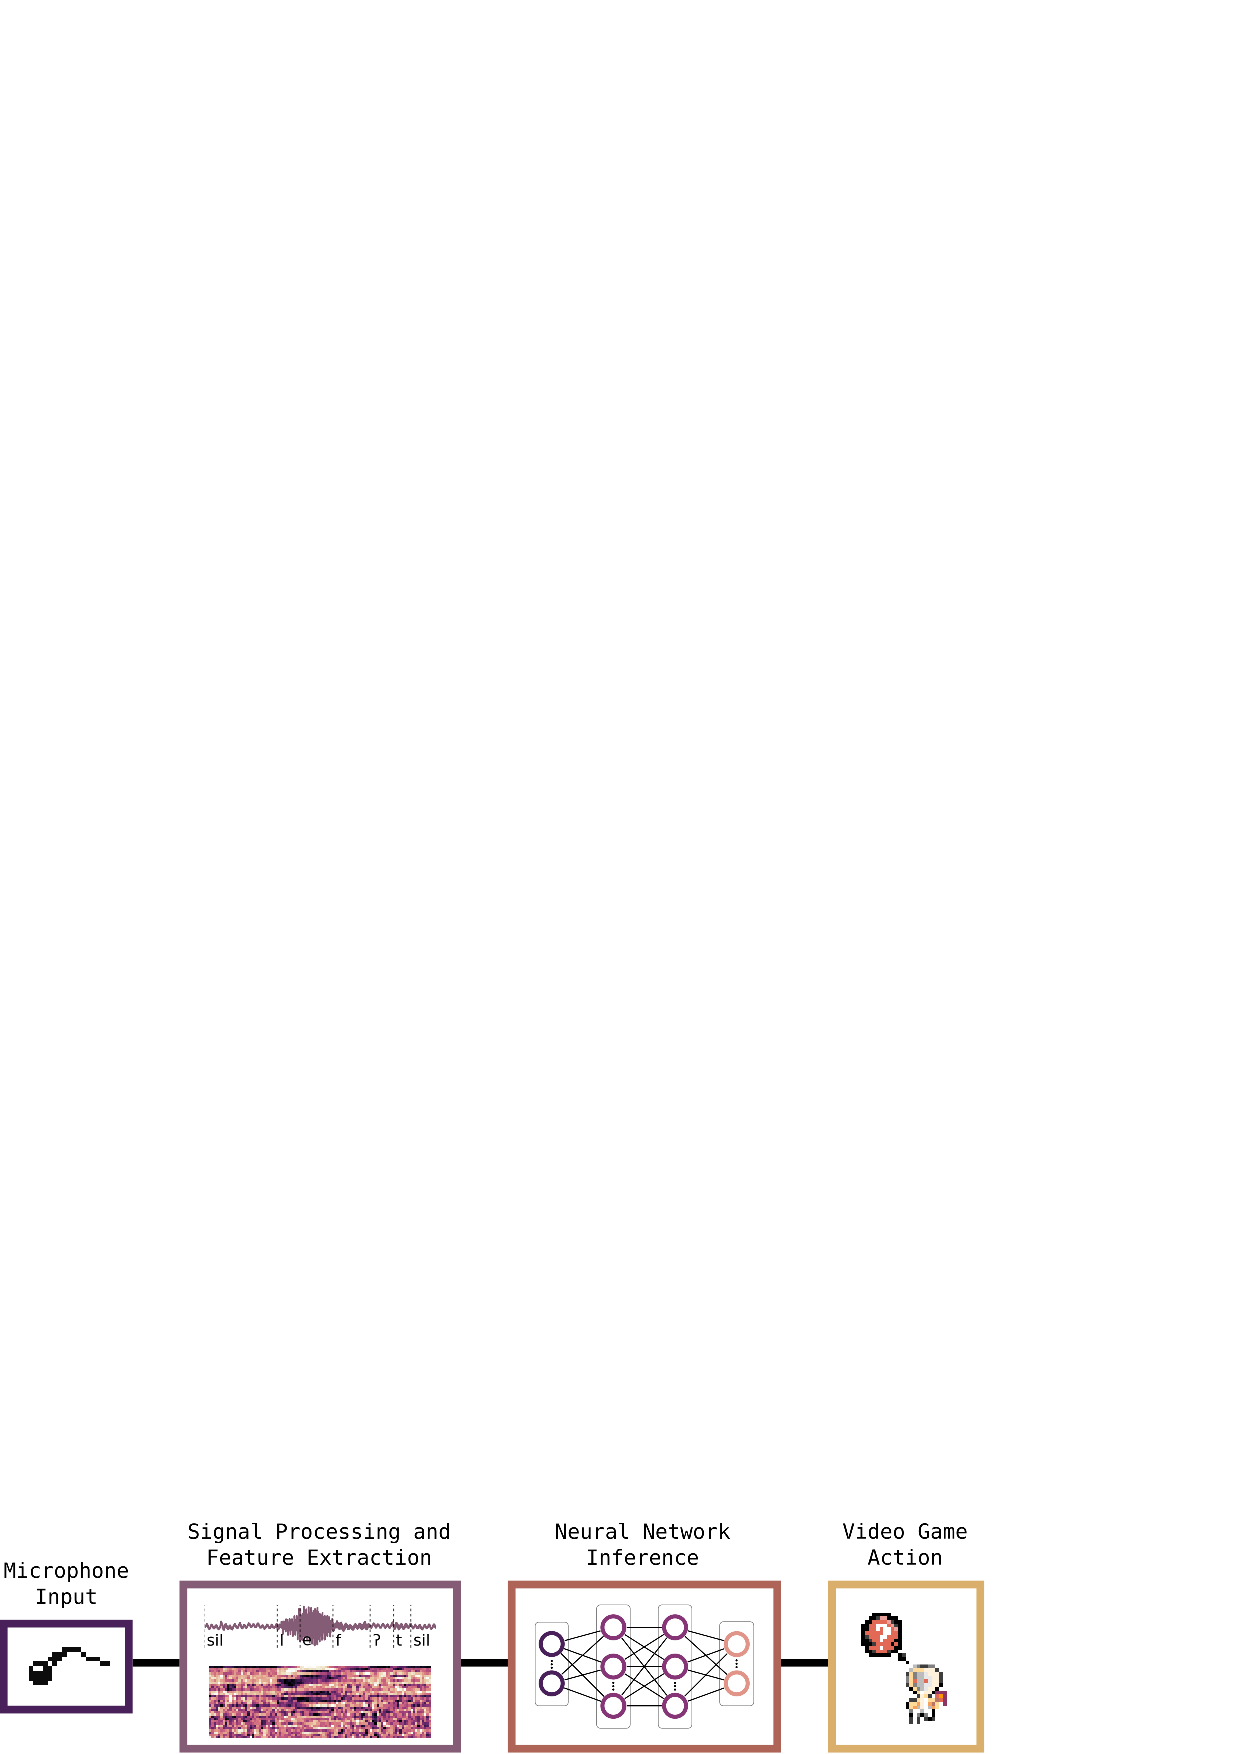
\includegraphics[width=0.95\textwidth]{./1_intro/figs/intro_kws.pdf}
  \caption{Simplified process of key word spotting for video games.}
  \label{fig:intro_kws}
\end{figure}
\FloatBarrier
\noindent
In the semantic perspective, the controlling of game objects, should be short, clear and best done with single command words, referred as speech commands.
Single words are easier to detect in comparison to long sentences, for instance, it is easier to recognize the word \enquote{left} than the sentence \enquote{missile target on position x, y}.
The classification of those speech commands can be done with a KWS system composed of a neural network.
KWS is restricted by a limited set of selected key words, referred as vocabulary or class dictionary.
In terms of video games, the set of key words might have members like \enquote{left} or \enquote{right}, for example, to move an element within the game to either left or right respectively.
The limited set of key words is crucial to restrict the complexity of the recognition task, since in practical applications it is not necessary to cover all words in a natural language.
Especially in video games, where the game environment is restricted by rules, technical limits and play-ability, KWS is suited perfectly as an alternative or augmented control system.
The size of the vocabulary and the selected words are two parameters that influence on one hand the choice of the neural network architecture, evaluated on energy efficiency and accuracy performance and on the other hand the game experience over the controls a player can choose from.
If the vocabulary of a KWS system would be too large, the chance of confusion between two different key words grows naturally.
In many KWS applications it is absolutely necessary to include labels for \emph{background noise}, \emph{silence} and \emph{unknown words} in the vocabulary. 
This is especially interesting in \emph{wake word} applications, where a single key word must be detected over the previously mentioned labels representing all other possible words that can be spoken.
Also in video games those additional labels are useful to prevent the player from eliciting unintended commands accidentally through, for instance, loud background noise.
Therefore, a KWS system has the demand of being very accurate and fast in its classification of key words.

Nowadays KWS systems are considered no science-fiction anymore, assisting consumers in everyday situations, such as rendering simple control tasks as the triggering of a photo release button on a \emph{smartphone} with a single speech command.
Application like this create more awareness of KWS, or generally speaking of speech recognition tasks, in human society.
Unfortunately some consumer applications with integrated speech recognition systems, leave a bitter aftertaste in data privacy issues and energy consumption through an externally and extensive computational processing pipeline over corporate servers \cite{Tang2018}.
It is therefore important to create incorporated KWS systems that respect private user data and provide an efficient implementation to save energy consumption.

Video games are a potential application for KWS, until now however, there exist very few of them taking advantage of this special feature.
Reasons for that might be found in the history of video games itself, where players find themselves in fast paced arcade games and speech recognition was simply too slow.
Additionally the complexity of KWS and lack of training data are often two valid arguments for not considering the deployment of a KWS system in a video game.

The following two sections in this introduction will briefly show the contributions of this thesis and give an overview of upcoming sections.
In summary, the focus of this thesis lies on KWS with neural networks trained through supervised learning on a speech command dataset \cite{Warden2018}.
The best suitable solutions for speech commands classification in video games are presented and evaluated with special interests in Convolutional Neural Networks (CNN), Generative Adversarial Neural Networks (GAN), and Wavenets.

% contributions
% --
% contributions

\section{Contributions}
The most of the effort is put into evaluating Convolutional Neural Network (CNN) models with low computational footprints, such as in \cite{Sainath2015}.
Besides low computational footprint, the depth of layers is hold to a minimum, so that it is still possible to get information about feature maps from the trained CNN networks.
The dataset used for the Key Word Spotting (KWS) task of those networks, was the speech command dataset \cite{Warden2018}.
The input features of the CNN models are the Mel Frequency Cepstral Coefficients (MFCC).
The amount of MFCC cepstral coefficients was evaluated with either 12 or 32 cepstral coefficients and showed that no accuracy improvements are achieved with 32 cepstral coefficients compared to 12.
The enhancement of MFCC to 39-feature vectors with 12 cepstral coefficients was also evaluated and showed only small improvements of accuracies, but not significant ones.
A frame-based normalization was performed on MFCCs to suite them better for visualization and use them for Generative Adversarial Networks (GAN) training.
Evaluation of the frame-based normalization was done in terms of accuracy, shift and noise invariance on conventional CNN models.
Frame-based normalization showed significant worse accuracies (about 5 to 10\%), it takes a bit longer for training, but improved in many experiments the noise invariance properties than without.
From those experiments the 12 cepstral coefficients with frame-based normalization were picked for further experiments.

Another large evaluation topic was that of GANs. 
With frame-based normalization the Generator (G) network was able to create convincing fakes to fool the Discriminator (D) network.
However it was found, when G and D are trained for too long, an equilibrium state where both generate random guesses or fakes might happen and the result is noise samples from G and a discrimination of D with slight changes around $0.5$.
Therefore a second loss term for G was added to create samples that have some similarity measure to the input data.
This helped to create better fakes and did not lead into noisy equilibrium states.

From the adversarial training of GAN networks, it was evaluated how their obtained weights through training can contribute in CNN models for KWS of speech commands.
Transfer learning was used to, transfer the obtained weights from either D or G to the equivalent CNN model.
With this approach it was possible to significantly increase the accuracy performance with about $3\%$ with using weights from G.
It showed that the obtained weights of G from an adversarial training can be very valuable.

A completely different approach for KWS was the evaluation of a Wavenet \cite{Oord2016} model for classification.
However with the hope that without feature extraction, a low computational model can be used, turned out to be extremely false.
Wavenets need a huge amount of operations by processing each sample from the audio files of the dataset.
Further the performances turned out to be very bad.
Nevertheless this model is evaluated and results are provided in hope for future research.

% overview
% --
% intro overview of thesis

\section{Overview of this thesis and notations}\label{sec:intro_overview}
\thesisStateReady
%This thesis is organized such, that each chapter leads to the next one and guiding someone who is interested in creating her own KWS game to follow through the process and challenges that might appear.
This thesis is organized that each chapter connects to the next one in a typical processing stage to create a KWS game.
% prev
After this introduction, \rsec{prev} provides information about previous and related work.
A small history sections about neural networks is given and important works on neural network architecture regarding this thesis are referrenced.
Further some works are presented that influenced and motivated this thesis.
Others works provide benchmarks on the used speech commands dataset or describe neural networks models that perform well on speech.
%In any way it is important to know, what is happening in the field of KWS and in which direction research is heading towards.
%Some works are used as motivation and some to get an idea.
% signal
\rsec{signal} is about audio signals processing and the extraction of meaningful features, such as MFCCs.
The feature extraction is explained in detail and examples are shown to visualize the results.
% neural networks
The used neural network architectures are described in \rsec{nn}. 
Further some theory of neural networks in general, CNNs, GANs and Wavenets is provided and highlighted with training results from experiments.
% experiments
In the \rsec{exp} information about the dataset and feature extraction is given and the experiments are presented.
Experiments are done on feature selection to determine the best suitable feature constellation the further experiments.
Adversarial pre-training is evaluated and Wavenets are compared to results from CNN based architectures.
% game
\rsec{game} describes the online and classification scheme in a possibile video game application.
Further some game design is presented and everything that is important for a KWS video game.
% conclusion
The thesis finishes with the conclusion in \rsec{conclusion}.


% visual guidance
%\subsection{Visual Guidance}\label{sec:intro_overview_visual}
%To get a better overview on the presentation of data and results, context specific color color-schemes are used within this thesis.
% There exist following context abstractions:

% \begin{itemize}
%     \item raw waveforms from soundfiles
%     \item extracted features, e.g. MFCCs
%     \item weights matrices of neural network models
%     \item training scores
% \end{itemize}

% ipa
\subsection{International Phonetic Alphabet}\label{sec:intro_overview_ipa}
The International Phonetic Alphabet (IPA) defines phonetics by human speaking sounds, where each symbol represents one specific sound.
A word formed with letters from a language alphabet, does not necessaryily represent the pronunciation of that word, therefore many dictionaries provide an IPA transcription so that no misconceptions may happen.
The plots, in some sections within this thesis, contain phonetic transcriptions with IPA characters, some of the more special ones are described in \rtab{intro_overview_ipa}.

% ipa table
\begin{table}[ht!]
\begin{center}
\caption{Some IPA and silence symbol with description.}
\begin{tabular}{ M{2cm}  M{9cm} }
\toprule
\textbf{IPA Symbol} & \textbf{Meaning} \\
\midrule
\textturnv & back vowel: \enquote{A}, open-mid roundend mouth \\
\textupsilon & back vowel: between \enquote{O} and \enquote{U}, nearly closed rounded mouth\\
\textinvglotstop & glottal stop\\
\midrule
sil & silence, no ipa symbol!\\
\bottomrule
\label{tab:intro_overview_ipa}
\end{tabular}
\end{center}
\end{table}
\FloatBarrier
\noindent



% math
\subsection{Mathematical Notations}\label{sec:intro_overview_math}
The mathematical equations or expressions are following some criteria.
Vectors and scalars are usually written in small letters with no special indication for vectors and matrices are written in capital letters.
The dimension of vectors and matrices are usually provided, such as $x\in\R^n$ or $X\in\C^{m \times n}$, or follow from the context.
Many letters like $n$ or $x$ are likewise used in different sections, but with different meaning and representations and should hopefully not confuse the reader of this thesis.
The letters $m$ and $n$ usually describes the length of a signal, $x$  and $y$ often represents input and output variables, etc.


% --
% background section

\chapter{Background}\label{sec:back}
This section provides fundamental background information regarding KWS, neural networks and video games.
The KWS task is described mathematically to express the actual speech recognition problem.
Notes on neural networks explain common properties and terms in their application.
Research questions are listed and give a deeper insight in common challenges of implementing a KWS system into a video game.

% disciplines
% --
% Intro of key word spotting

\section{The Key Word Spotting Task}\label{sec:intro_kws}
\thesisStateRevised
As described in \rsec{intro}, KWS is the task of classifying speech signals of spoken words to single key words out of a set of key words.
The set of key words $S$, also called vocabulary, can be defined as:
% kws dict
\begin{equation}\label{eq:intro_kws_dict}
	S \coloneqq \{s_i \mid i = 0, 1, \dots, L\}
\end{equation}
with a total number of $L$ key words denoted individually as $s_i$ for each key word.
The task is to select the key word closest to the spoken word from the user, denoted as target $t$.
The target does not necessarily have to be a member in the set of key words $S$, in fact it can be any arbitrary word.
With the abstract formulation:
% kws task
\begin{equation}\label{eq:intro_kws_task}
	\hat{s} = \underset{s_i \in S}{\arg \min} \, \mathcal{D}(t, s_i)
\end{equation}
the most probable key word $\hat{s}$ can be predicted, where $\mathcal{D}$ is some kind of distance measure between two words.
The formulation in \req{intro_kws_task} is merely semantic, but KWS in computer systems must cope with various transformations of raw input samples of audio data denoted as $\bm{x} \in \R^n$, with a total number of $n$ samples.
From the audio data an inference to output class probabilities $\bm{y} \in \R^L$ with a total number of $L$ class labels or key words, can be processed for instance with a neural network containing a softmax function at its last layer (transforming the output of the last layer to probability values).
With the softmax output from a neural network, the most probable key word can be picked by:
\begin{equation}\label{eq:intro_kws_class}
	\hat{s} = \{s_i \mid \underset{i = 0, 1, \dots, L}{\arg \max} \, y_i\}
\end{equation}
if the highest value of $y_i$ for all $i$ refers to the most probable index or indices of a spotted key word or key words in the vocabulary.

In comparison to full Automatic Speech Recognition (ASR), where whole sentences need to be identified, key word spotting operates merely on the word level.
Therefore KWS is a bit easier to deploy and less complex than ASR.
On the other hand KWS systems, that are used in practical applications, must run very energy efficiently on low energy devices, such as mobile phones, and give immediate and accurate responses to the users. 
A good elaboration on the requirements of KWS systems can be found in the motivation section of \cite{Warden2018}.
% --
% Intro to neural networks

\section{Neural Networks for Key Word Spotting}\label{sec:intro_nn}
\thesisStateReady
Neural networks enable computers to automatically learn from data to be able to solve tasks such as pattern recognition in images or audio.
The examples or samples from the input data can be paired with annotations, denoted as \emph{labels} or \emph{classes}.
If the label information of each example is used during the \emph{training} of a machine learning system, such as a neural network, it is called \emph{supervised learning} otherwise it is called \emph{unsupervised learning}, however supervised learning is more commonly applied.

%The big advantage of neural networks is that they are able to cope with huge amounts of input variables per data example and are able to extract their own features of those inputs through many layers within the network.
The big advantage of neural networks is that they are able to cope with large amounts of input variables per data example.
Considering a raw waveform file of merely \SI{1}{s} time duration, sampled with \SI{16}{\kilo\hertz} would give a input size of 16000 features.
This huge amount of input features is even difficult for neural networks to learn from and usually a feature extraction stage is placed in between to reduce the input dimension.
For instance the computation of MFCCs, using 12 out of 32 coefficients and a time duration of \SI{0.5}{s} with a time shift of \SI{10}{\milli\second}, reduces the input feature size dramatically to $12 \times 50 = 600$, which is still a high number of input features, but much more affordable and faster to train.

%In this thesis, the word \emph{feature} has several meanings, one is as name of extracted data and therefore be the same as input variables. 
%Another is, that a feature is simply some kind of compressed representation of a high dimensional data.
Neural networks are able to learn own feature representations, selection and interpretation, rather than using hand-crafted ones done by humans with expertise in the application.
Note that hand-crafting features of a complex recognition task, is in most cases not even possible or extremely cumbersome.
So researchers prefer neural networks because of their easy deployment scheme and state of the art performances.
Further it enables everyone who is capable of using neural network tools, to create solution to rather complex problems usually solved by experts in the field, given there is enough data and processing power available.
Therefore elaborate feature extraction stages become less important to the users.
This on the other side may lead into less understanding of the actual problem and more \enquote{try and error} approaches of different neural network architectures and training parameters.
The energy consumption required to train large neural network with many parameters on a huge training dataset, shall not be forgotten, especially in times of climatic change.
Reusing pre-trained weights from renowned network architectures is a good way to reduce energy consumption in finding an optimal classifier for a specific task.
The re-usability of pre-trained weights is often named as \emph{transfer learning}. 
A small summary on transfer learning can be found in \cite{TransferLearning}.
%This led to the thinking that everyone, who owns data and computational power, is the superior of solving complex problems such as image or audio classifications.
%However it is not always like this rather negative example, when using neural network approaches.

The potential of neural networks in research are vast.
The observation on how the learning from data is done and what recognition patterns are obtained after training, might allow researchers and experts to better understand the problem or gain a different viewpoint on it.
%However if neural networks are observed on how they are able to learn from data and what recognition patterns they have obtained after training, it might benefit researchers and experts to better understand the problem or gain a different viewpoint on it.
%It is extremely interesting to work with them and get knowlege about how and why they are able to produce such good results.
%This again feedbacks experts to gain more understanding or a different viewpoint on the topic.
Especially when using Convolutional Neural Networks (CNN), researchers are actually able to observe and visualize the learned filters and interpret the results.
A very interesting example of investigating learned CNN filters is shown by Zeiler el. al. \cite{Zeiler2013}.
Other interesting subjects in research are generative models, such as Generative Adversarial Networks (GAN) \cite{Goodfellow2014}, which are able to create convincing samples from the learned data distribution.

Neural network architectures for speech recognition are a little bit different from image recognition, mainly because of the sequential nature of time signals.
However if time signals are restricted in time, that means limited to a fixed number of samples, and frequency features are extracted over that time span, then speech signals can be represented in 2D space (frequency and time) and classified like images.
That suggests that CNNs are reasonable network architectures for speech as well.
Another interesting architecture for audio signals is the Wavenet \cite{Oord2016}, because of its ability to process raw audio data.
%and were originally intended for speech synthesis, but could also be used for recognition tasks.



% --
% video games with speech commands

\section{Video Games with Speech Input}\label{sec:intro_games}
\thesisStateReady
Video games with speech inputs are a rarely seen occurrence in the gaming industry, though it is a very interesting and immersive way to interact.
Technically the voice of the player of the video game, has to be recorded by a microphone, therefore one additional requirement of being able to play the video game is to own a microphone, which however does not need to be high-end.
The input stream of a microphone can be processed through an online or realtime system to extract the input data for the classification system.
The classification system, such as a neural network, infers the input data and therefore hopefully the intention of the player to a real action within the game.
The processing scheme is easy to define, but not that easy to implement compared to other more hardware based input channels, such as a click on a keyboard button.
Also speech input is very slow compared to hardware input, where players interact within tens of milliseconds (the input lag of gaming controllers should ideally be under \SI{50}{\milli\second}).
This is not possible with speech, the player has to physically form a waveform representing the action in the game.
Further the waveform captured from the online system has to be pre-processed, feature extracted and classified to the best estimation of all the available key words in the games vocabulary.
Concluding this, a good estimate to create and process a speech input should ideally be under one second, the less the better for the playing experience.

Another important question is how many key words or speech commands, should be used for the vocabulary.
A high number of key words will increase the chance of confusion and a small number of key words restrict the possible actions a player can choose from.
The possibility to create separate classifiers with different sets of smaller vocabularies of speech commands arises depending on which commands the player actually needs in the actual scenario within the video game. For instance if the player is in a dialogue with a Non Player Character (NPC) it makes sense to reduce the vocabulary to only \{\enquote{yes}, \enquote{no}\} if those are the only actions to choose from.

The use of labels for background noise, silence and unknown words depends on the game and how the classification process is activated.
If the assumption is made that a player chooses only from the key words in the dictionary, then the label of unknown words is not really necessary.
However the unknown label would be very interesting if key words are not that common to a player, such as words from a different language or fantasy words.
The unknown label will therefore motivate the player to correctly pronounce the word itself, which could be also used in language learning games.
The labels for background noise and silence are useful if the activation of the classification process is initiated by the energy value of the input stream of the microphone.
A stroke on the microphone or loud background sound can therefore elicit an unwanted command within the game, if those labels do not exist.

In any case there are much problems to consider when using KWS in video games and probably therefore hinders game developers to produce more content with it.

%Maybe those issues and the complexity of the task hinders game developers to produce more content with Key Word Spotting.
% A speech input for video games is a spoken waveform, recorded through a microphone, from any speaker intending to inflict a certain change while playing a Video Game. 
% Certainly this spoken waveform has to be processed, such as other inputs channels have to be (like keyboard buttons pressed), so that its meaning can be understood by the computer system behind the game. 
% Although this processing of a waveform is much more complicated and prone to errors, compared to a simple click on the keyboard or mouse. 
% That might be one of the reasons why Speech Inputs are very rare to be found in Video Games, still they exist.

% research questions
% --
% research questions

\section{Research Questions for this Thesis}\label{sec:intro_rq}
This section formulates relevant research questions regarding KWS in video games.
Those research questions can be split into 3 parts:
\begin{enumerate}[label={Q.\arabic*)}, leftmargin=1.4cm]
  \item Signal processing and feature extraction of speech signals.
  \item Neural network training and classification for KWS.
  \item Video games with KWS.
\end{enumerate}
Note that the terms \enquote{key word} and \enquote{speech command} are often named interchangeably because speech commands are used as key words in the KWS system.
Not all research questions can be answered within the scope of this thesis.
Nevertheless, those questions can be asked and some solution concepts discussed.


% --
% signal

\subsection{Signal Processing and Feature Extraction Research Questions}\label{sec:intro_rq_signal}
Acquiring meaningful features from speech signals is essential for neural networks to operate on. 
The features are extracted from raw audio samples of a microphone input stream in a specific time interval.
Those retrieved features are further input to a neural network for the classification of speech commands.
The following Questions arise here:
\begin{enumerate}[label={Q.1.\alph*)}, leftmargin=1.75cm]
  \item Which time interval should be captured to represent a speech command?\label{it:q1-a}
  \item Does the signal processing have to be invariant to background noise and especially to game sounds?\label{it:q1-b}
  \item What are meaningful features for speech recognition?\label{it:q1-c}
\end{enumerate}
\noindent
\textbf{Question \ref{it:q1-a}:} 
The time required to fully pronounce a speech command is not fixed and varies from speaker to speaker, depending also on the intended prolongation a speaker adds to the word.
In practical applications however, a fixed time interval for a single speech command is convenient.
By restricting the time duration of the key words, the speaker has to pronounce the words within this time span.
For example, if a speaker pronounces the word \enquote{left} and requires a time duration of \SI{1}{\second}, hardly all is captured if the time interval is restricted to merely \SI{500}{\milli\second}.
Whether this \SI{500}{\milli\second} is sufficient for a correct classification, is subject for evaluation.
In the application of a video game, the user should preferably speak the commands with a short time duration so that the game can respond fast.
Problems might occur if the speech commands are spoken repeatedly and very hasty such that the time interval of consecutive commands overlap each other.
Ideally the time interval to represent a speech command would be flexible but this more difficult to implement than a fixed time interval.

\textbf{Question \ref{it:q1-b}:}
Usually the presence of low background noise should not be a problem for neural networks trained on a large enough data set. 
The game sounds might present a more difficult problem, when turned up too loud without the use of headphones. 
Therefore, the microphone will not only capture the voice of a speaker but also a fair amount of game sounds. 
This problem seems to be theoretically solvable as the shape of the nuisance is known and the amount of game sound in the audio stream could be attenuated sufficiently.
In practice this might be hard to solve without critically disturbing the signal of interest.
A solution to this problem would probably take too much time and effort and is therefore not evaluated within this thesis. 
However, playing a video game without game sound is unsatisfying and it would be a great contribution to tackle this problem in future work.

\textbf{Question \ref{it:q1-c}:} 
The determination of meaningful features for speech signals is a classical problem in speech recognition.
The essential composition of a word may help to understand the problematic better.
A word is a sequential combination of either vowels, such as \enquote{a} and \enquote{e}, or consonants \enquote{k}, \enquote{l}, with a certain length. 
In linguistics, for instance, it is possible to distinguish vowels with frequency peaks in a spectrogram, where a spectrogram is the magnitude squared of the frequency response of small time chunks over the time duration of a signal.
However, due to many different factors in voice generation involved in speakers, such as age, gender, nationality and physiology of the vocal tract, there is a huge variance in the pronunciation of words from different persons, which increases the difficulty of the problem.
A very common approach is to use MFCCs as features for speech recognition tasks.
Why MFCCs present reasonable features for speech, is described in detail in \rsec{signal_mfcc}.


% --
% neural networks

\subsection{Neural Network Implementation Research Questions}\label{sec:intro_rq_nn}
Neural networks for video games should ideally be very efficient and provide accurate classifications of input features.
The vocabulary in a KWS task has to be specified for the individual game and chosen from all class labels available in the dataset.
Each key word of the vocabulary is presented by one output node of the neural network architecture.
Following Questions can be asked in general:
\begin{enumerate}[label={Q.2.\alph*)}, leftmargin=1.75cm]
  \item Is there an appropriate dataset suited for KWS video games and with sufficient diversity available?\label{it:q2-a}
  \item What happens if an input feature represents a spoken word, which is not in the vocabulary (unknown key word) and how should this exception be handled?\label{it:q2-b}
  \item What is the best neural network architecture regarding classification accuracy and energy efficiency?\label{it:q2-c}
  \begin{enumerate}[label=(\roman*)]
    \item Can adversarial networks improve generalization?
    \item Are Wavenets a solution to this task?
  \end{enumerate}
\end{enumerate}
\noindent
\textbf{Question \ref{it:q2-a}:} 
The availability of a dataset for KWS video games can be answered right away, as there exists a speech commands dataset \cite{Warden2018} with enough and diverse data.
The dataset consist of 35 labels and contains commands for movement and numbers.
Further, it includes randomly selected words like \enquote{marvin} or \enquote{bird} intended to represent \emph{unknown} words for the KWS system.
It has to be noted that not every game idea can be realized with a restricted vocabulary.
Nevertheless, with commands for movement like \enquote{left} or \enquote{go} it is possible to move objects within a game and this can already be used for many game mechanics.
An aspect regarding efficiency, is to restrict the amount of key words in the vocabulary as much as possible such that a cheaper neural network architecture can be deployed, which of course should still be sufficiently good in its classification accuracy.

\textbf{Question \ref{it:q2-b}:} 
Without doubt, players will try out words that are not in the vocabulary (denoted as \emph{unknown} key words) and observe the response of the video game.
The ideal response would be to shown an indication to the player that the word is not present in the vocabulary. 
Nevertheless, it might happen that the similarity of an unknown key word is too close to a key word and an unintended action is triggered in the game. 
At the same time the neural network should not classify key words as unknown key words to ensure a satisfying game experience.
It is better to rely on that players are using key words for most of the time so that they are preferred over unknown key words.

\textbf{Question \ref{it:q2-c}:}
In the ideal case, video games with KWS do not slow down during the inference process of unknown input data.
The restriction of the amount of computations and time for the classification of key words is given by the minimum Frames Per Second (FPS) a video game is perceived as fluent.
That requires the FPS to not fall under a certain limit (usually 30 FPS in video games), otherwise the fluidity of the game is not guaranteed.
Therefore, several different neural network approaches with a low computational footprint have to be tested and compared against each other regarding classification rate and energy efficiency.
The transfer of weights from GANs is an interesting approach to evaluate whether the trained parameters are also useful for pure classification tasks in CNNs.
Wavenets have the advantage that they do not need a feature extraction stage but it is questionable whether the network design achieves a reasonable computational footprint.


% --
% video games

\subsection{Video Games with KWS Research Questions}\label{sec:intro_rq_games}
Video games that use KWS can create an unique playing experience but have to face certain challenges.
Following questions can be stated:
\begin{enumerate}[label={Q.3.\alph*)}, leftmargin=1.75cm]
  \item How should the onset of a key word be detected, so to reduce computations?\label{it:q3-a}
  \item What is the added value of KWS in the gaming experience of players?\label{it:q3-b}
  \item What do game developers have to consider, when designing a game with KWS?\label{it:q3-c}
\end{enumerate}
\noindent
\textbf{Question \ref{it:q3-a}:} 
It is crucial to reduce computations in a video game in order to keep it running fluently during high performance peaks.
Also the unnecessary processing of meaningless input data should be avoided as much as possible.
Ideally the key word classification is activated, when there is actually a speech command present, which however is not always trivial.
One possibility to indicate the onset of a key word is to perform the relatively efficient calculation of an energy value within a certain time interval of the raw input data stream and have a simple threshold value decide, whether a speech command is available. 
To avoid the consecutive triggering of onsets at each energy measure, the microphone and amplifier noise floor and the background sound (including the game sound) have to be less energy intensive than the speech signal obtained from the player.
Another approach similar to the push and talk principle, would be to indicate the onset of a key word with the click of a certain button on the keyboard.
The player is therefore able to control the exact onset of a key word and its length but requires an additional hardware based input channel.

\textbf{Question \ref{it:q3-b}:}
In certain video game scenarios, speech commands can be useful, interesting and enhancing for the gaming experience, in others they might even disturb the game play or even spoil it completely.
It cannot be generally stated whether it is worth to deploy a KWS system into a game, this depends on the game it is intended for.
As already noted in \rsec{intro_games}, KWS might be a great augmented control system for special kind of games to increase the immersion experience, especially for VR applications.
Also language learning games are an interesting application but usually require a huge vocabulary and therefore a phoneme based ASR system would be the better choice.

\textbf{Question \ref{it:q3-c}:}
Apart from the technical requirements involved in KWS systems, also the general game design with KWS has to be considered.
It certainly can be stated that KWS systems are not always reliable and therefore a main game mechanic solely based on it is not always preferred.
Furthermore, the time lag required to process speech commands to actual actions within the game should not be ignored.
The player should get on the one hand immediate and accurate feedback from the game and on the other hand be challenged while playing.
Further, by achieving both criteria it ensures that the game experience does not suffer from getting frustrating or tiresome.
Additionally it must be considered, that players might get exhausted by using speech commands consecutively in short intervals during the game.
Therefore, the players might prefer a game design where they have to use KWS only in special situations.
As general conclusion, it can be stated that a game developer has to design a KWS game with great care.
% --
% previous and related work

\chapter{Previous and Related Work}\label{sec:prev}
This chapter presents important works that had influenced this thesis.
The works can be separated in audio features, neural networks, key word spotting and video games with key word spotting.

% features
% --
% prev features

\section{Audio features}
The extraction of audio features from acoustic waveforms is important for data compression.
One of the most popular features are the Mel Frequency Cepstral Coefficients (MFCC), developed by
\cite{Mermelstein1980} in 1980.
They are motivated by the physiological human hearing system.

% neural networks
% --
% prev neural networks basics

\section{Neural Networks Basics Architectures}\label{sec:prev_nn}
\thesisStateNotReady
This section is a summary and history review of some specific neural network architectures used within this thesis.
The purpose is merely to give a slight overview of these architectures and the researchers that contributed to them.

% --
% prev history

\subsection{Historical Remarks on Neural Networks}\label{sec:prev_nn_history}
The first step towards computational neural networks, as we know them today, was the introduction of the so called \enquote{Perceptron} by Rosenblatt in the year 1958 \cite{Rosenblatt1958}. 
The idea of the Perceptron emerged from physiologists, trying to model a physiological neural network in computational terms. 
This first model was based on the information processing of the retina (input nodes), which passes through several physiological neural networks (hidden nodes) and finally elicit an action or decision (output nodes).
Publishing his work and implementing those ideas in an actual computer system (at those time computers were huge boxes), Rosenblatt kicked of the domain of computational learning systems.
The race of finding best neural network architectures for specific regression or classification tasks had begun.

Another big advance in the history of neural networks, was the introduction of a very famous learning algorithm known as \enquote{Backpropagation}, evolved by several authors at the same time \cite{LeCun1986} and \cite{Rumelhart1986} in the late 80s. 
Even nowadays, 35 years after introducing backpropagation, it is still the \emph{de facto} standard in training neural networks.
Nowadays backpropagation is implemented in every machine learning framework for neural networks as its core element.
Such frameworks are for instance \texttt{Pytorch} or \texttt{Tensorflow} and of course many others, handling the gradient calculation and backpropagation algorithm of those gradients in the background.

The neural networks reputation during the time until now, was not always seen that splendid.
The general problem of handling overfitting (prevent networks from learning data samples by heart) and generalize better on unseen data, is still an open issue in many applications.
Some mathematicians working in the field of statistical methods in learning theory for pattern recognition, regard neural networks as being not meaningful in the advance of learning theory, such as one quote from \cite{Vapnik1995} of Vapnik's book in 1995 about natural learning theory:

\begin{quote}
...In spite of important achievements in some specific applications using neural networks, the theoretical results obtained did not contribute much to general learning theory...
\end{quote}

This quote is a bit tough, but unfortunately true in some sense. 
The complexity of neural networks with many layers, makes the tracing of the learning process very difficult.
No concrete formulas, apart from the calculation of gradients, can exactly explain what neural networks are actually learning.

Therefore on one side there were the classical statistical learning methods, the most famous one called Support Vector Machines (SVM) \cite{Cortes1995} and one the other side there were neural network approaches.
Over a long period of time SVMs were preferred over neural networks, because they were better understood with profound mathematical methods and achieved state of the art performance with sophisticated feature extraction algorithms.
Not until 2012, neural networks gained more popularity again by scoring new benchmarks in image classification tasks with one famous paper \cite{Krizhevsky2012}, by beating the previous benchmark with a significant score.
Deep Learning was the new key to success, with network architecture consisting of many layers and a large amount of parameters to train.
Also in audio and language processing tasks, such as Automatic Speech Recognition (ASR) and Natural Language Processing (NLP), the famous Hidden Markov Models (HMM) and other statistical methods get more and more replaced by neural networks.

With this remarks the short review on neural network history are closed and readers may forgive that not more details are presented and more papers referenced.
The interested reader is recommended to look through the references of the above mentioned papers for finding more detailed informations about its interesting history.


% --
% convolutional nets

\subsection{Convolutional Neural Networks}\label{sec:prev_nn_cnn}
Convolutional Neural Networks (CNNs) are a special class of neural networks, that are able to incorporate spatial information from the input data, with the application of convolutional filtering to create feature maps.
Spatial information is very important in images, where neighboring pixels are related to each other.
The same holds for audio, but in only one dimension and with a higher amount of samples.
Convolutional filters are very commonly applied in image processing tasks, such as denoising or other enhancements of images.
In audio processing, a classical application of convolutional filters is a simple average filter of the signals energy, to determine onsets like the start of a speech signal.

Still it took relatively long till convolutional filters were a common and a widely used asset in neural network architectures.
The general concepts of CNNs with feature maps (outputs of applied convolutional filters) and weight sharing through convolutional filters, were examined by LeCun et. al. on handwritten postal codes in 1989 \cite{LeCun1989_Generalization}.
Further research and experiments on the famous MNIST dataset of handwritten digits, were done in the late 90s \cite{LeCun1998} and asserted the success of CNNs.
A classical convolutional layer in CNNs usually consists of multiple convolutional filters with trainable weights and an additive bias terms per filter, followed by a non-linear activation function.
More details about CNNs is presented in
%Since then many famous image recognition models were introduced that incorporated CNNs and achieved state of the art performances.

%This is one reason why CNNs are so practicable for image recognition tasks and usually state of the art image recognition architectures have some kind of convolutional neural network implemented within.

%With their restricted and highly spatial connections and weight sharing through convolutional filters, they are an valuable asset no researchers should miss when working with images or audio recognition.

  
% best quote ever
%It is trivial to design a machine that learns very quickly, does not generalize, and requires an enormous amount of hardware. 
%In fact this learning machine has already been built and is called a Random Access Memory.


% --
% recurrent neural networks

\subsection{Recurrent Neural Networks}\label{sec:prev_nn_rnn}
Recurrent Neural Networks (RNN) are a type of neural networks, that are using feedback loops from the output of each node back to its input.
With those feedback loops it is possible to input sequential data with no fixed length restrictions.
%The information state is stored within the network.
RNNs are known to be hard to train because of the well known exploding or vanishing gradients problem.
This problem can be solved by using so called Long Short Time Memory (LSTM) that are incorporating gates for the information storage in each cell. 
However the LSTM cell also increases the amount of parameters to be trained for each node and backpropagation over a large amount of time steps is computationally intensive.

Through their design to capture sequential data, RNNs are commonly used in speech recognition tasks.
However they are not subject in this thesis, the interested reader if referred to a good comprehension in \cite{Staudenmeyer2019} with further references upon RNN works.


% --
% wavenets

\subsection{Wavenets}\label{sec:prev_nn_wavenet}
Processing raw audio data as inputs to neural networks seemed to be difficult for a long time.
This is mainly due to their huge amount of input data. 
Consider a \SI{1}{\second} audio file with a sampling rate of \SI{16}{\kilo\hertz} give 16000 samples and therefore a 16000 dimensional input vector.
Recently neural network architectures emerged with the ability to process raw audio samples.
One very prominent architecture, originally intended for natural speech generation, is the so called \emph{Wavenets} \cite{Oord2016}.

With the \emph{dilated convolution} and a quantization of the audio sample values, Wavenets can afford to process this huge amount of inputs.
Wavenets are in some sense similar to RNNs, because they also use outputs from previous time steps, but the implementation of wavenets is much more efficient, such as the quote from \cite{Oord2016} states:
\begin{quote}
  %Recurrent neural networks such as LSTM-RNNs (Hochreiter & Schmidhuber, 1997) have been a key component in these new speech classification pipelines, because they allow for building models with long range contexts. 
  ...With WaveNets we have shown that layers of dilated convolutions allow the receptive field to grow longer in a much cheaper way than using LSTM units...
\end{quote}


% --
% adversarial nets

\subsection{Generative Adversarial Neural Networks}\label{sec:prev_nn_adv}
Generative Adversarial Neural Networks (GAN) are motivated by Game Theory, in a way that they contain usually two separate networks, denoted as players, playing a game against each other.
The game hereby is to outperform the other player in an adversary task.
The idea of GANs emerged from Goodfellow in 2014 \cite{Goodfellow2014}, where one player (network) produces fake images, that are similar to real ones and the other player has to detect if it given image is a real or fake one.
Both players are therefore improving themselves upon each other, to either create more realistic fakes or to detect fakes from reals with low error rates.

In this thesis, the concept of GANs is used for pre-training weights to hopefully improve generalization and performance in a CNN network.
% --
% prev history

\subsection{Historical Remarks on Neural Networks}\label{sec:prev_nn_history}
The first step towards computational neural networks, as we know them today, was the introduction of the so called \enquote{Perceptron} by Rosenblatt in the year 1958 \cite{Rosenblatt1958}. 
The idea of the Perceptron emerged from physiologists, trying to model a physiological neural network in computational terms. 
This first model was based on the information processing of the retina (input nodes), which passes through several physiological neural networks (hidden nodes) and finally elicit an action or decision (output nodes).
Publishing his work and implementing those ideas in an actual computer system (at those time computers were huge boxes), Rosenblatt kicked of the domain of computational learning systems.
The race of finding best neural network architectures for specific regression or classification tasks had begun.

Another big advance in the history of neural networks, was the introduction of a very famous learning algorithm known as \enquote{Backpropagation}, evolved by several authors at the same time \cite{LeCun1986} and \cite{Rumelhart1986} in the late 80s. 
Even nowadays, 35 years after introducing backpropagation, it is still the \emph{de facto} standard in training neural networks.
Nowadays backpropagation is implemented in every machine learning framework for neural networks as its core element.
Such frameworks are for instance \texttt{Pytorch} or \texttt{Tensorflow} and of course many others, handling the gradient calculation and backpropagation algorithm of those gradients in the background.

The neural networks reputation during the time until now, was not always seen that splendid.
The general problem of handling overfitting (prevent networks from learning data samples by heart) and generalize better on unseen data, is still an open issue in many applications.
Some mathematicians working in the field of statistical methods in learning theory for pattern recognition, regard neural networks as being not meaningful in the advance of learning theory, such as one quote from \cite{Vapnik1995} of Vapnik's book in 1995 about natural learning theory:

\begin{quote}
...In spite of important achievements in some specific applications using neural networks, the theoretical results obtained did not contribute much to general learning theory...
\end{quote}

This quote is though, but unfortunately it is true in some sense. 
The complexity of neural networks make them not tractable in their learning process.
No concrete formulas, apart from the calculation of gradients, can exactly explain what neural networks are actually learning.

Therefore on one side there were the classical statistical learning methods, the most famous one called Support Vector Machines (SVM) \cite{Cortes1995} and one the other side there were neural network approaches.
Over a long period of time SVMs were preferred over neural networks, because they were better understood in their mechanism and achieved state of the art performance with sophisticated feature extractions algorithms at that time.
Not until 2012 neural networks gained more popularity again, scoring new benchmarks in image classification tasks with one famous paper \cite{Krizhevsky2012}.
Deep Learning was the new key to success, with network architecture consisting of many layers and a large amount of parameters to train.

Here this short review on history shall be stopped and readers may forgive that not more details are presented and more papers referenced.
The interested reader is recommended to look through the references of the above mentioned papers for finding more detailed informations.

% --
% prev convolutional nets

\subsection{Convolutional Neural Networks}\label{sec:prev_nn_cnn}
Convolutional Neural Networks (CNNs) are a class of neural networks, that are able to incorporate spatial information with the application of convolutional filtering.
Spatial information is very important in images, where neighboring pixels are releated to each other.
The same holds for audio, but in only one dimension and with a higher amount of samples.
Convolutional filters are very commonly applied in image processing tasks, such as denoising or other enhancement of images.
In audio processing, a classical application of convolutional filters is a simple average filter of the signals energy, to determine onsets like the start of a speech signal.

Still it took relatively long till convolutional filters were a common used asset in neural network architectures.
The general concepts of CNNs with feature maps (convolutional filters) and weight sharing through those feature maps
were examined by LeCun et. al. on handwritten postal codes in 1989 \cite{LeCun1989_Generalization}.
CNNs were introduced and examined by LeCun et. al. on handwritten digits of the MNIST dataset in the late 90s
\cite{LeCun1998}.
%Since then many famous image recognition models were introduced that incorporated CNNs and achieved state of the art performances.

%This is one reason why CNNs are so practicable for image recognition tasks and usually state of the art image recognition architectures have some kind of convolutional neural network implemented within.

%With their restricted and highly spatial connections and weight sharing through convolutional filters, they are an valuable asset no researchers should miss when working with images or audio recognition.

  
% best quote ever
%It is trivial to design a machine that learns very quickly, does not generalize, and requires an enormous amount of hardware. 
%In fact this learning machine has already been built and is called a Random Access Memory.

% --
% prev recurrent neural networks

\subsection{Recurrent Neural Networks}\label{sec:prev_nn_rnn}
Recurrent Neural Networks (RNN) are a type of neural networks, that use a feedback loop of their output over time.
It is therefore possible to store relevant input information over a fixed time span.
The neural network architecture can then be seen as unrolled over time.
However this unrolling multiplies the per time instance network architecture for each additional time instance,
which easily becomes a huge network.
Also RNNs are known to be hard to train because of exploding or vanishing gradients.
This problem can be solve with using so called Long Short Time Memory (LSTM) neural networks incorporating gates for the information storage in each cell. However the LSTM cell also increases the amount of parameters to be trained.
Through their design to capture sequential data, Recurrent Neural Networks are commonly used in speech recognition tasks.
However they are not regarded in this thesis because of being to cost intensive for a video game deployment.
The interested reader might read a good comprehension in \cite{Staudenmeyer2019}.


% --
% prev adversarial nets

\subsection{Adversarial Neural Networks}\label{sec:prev_nn_adv}
Adversarial Neural Networks are motivated by Game Theory, in a way that they incorporate usually two separate networks, denoted as players, playing a game against each other.
The game hereby is to outperform the other player in a specific task.
The idea of creating generative networks emerged from Goodfellow in 2014 \cite{Goodfellow2014}, where one player (network) produces fake images, that are similar to real ones and the other player has to detect if it given image is a real or fake one.
Both players are therefore improving themselves upon each other, to either create more realistic fakes or to detect fakes from reals with low error rates.

% --
% prev wavenet

\subsection{Wavenets}\label{sec:prev_nn_wavenet}

Processing raw audio data as inputs to neural networks seemed to be difficult for a long time.
This is mainly due to their huge amount of input data, consider a \SI{1}{\second} audio file with a sampling rate of \SI{16}{\kilo\hertz} yield into 16000 samples and therefore a 16000 dimensional input vector.
Recently neural network architectures emerged with the ability to process raw audio samples.
One very prominent architecture, originally intended for natural speech generation, are so called \emph{Wavenets} \cite{Oord2016}.

With a smart convolution technique called \emph{dilated convolution} and a quantization of the audio sample values, wavenets could afford to process this huge amount of raw audio inputs.
Wavenets are in some sense similar to RNNs, because they also use outputs from previous time steps, but the implementation of wavenets is much more efficient, such as the quote from \cite{Oord2016} states:
\begin{quote}
  %Recurrent neural networks such as LSTM-RNNs (Hochreiter & Schmidhuber, 1997) have been a key component in these new speech classification pipelines, because they allow for building models with long range contexts. 
  ...With WaveNets we have shown that layers of dilated convolutions allow the receptive field to grow longer in a much cheaper way than using LSTM units...
\end{quote}

% KWS for speech commands
% --
% prev key word spotting

\section{Key Word Spotting with Neural Networks}\label{sec:prev_kws}
\thesisStateNotReady
Some important works regarding KWS with neural networks are presented here. 
The aspect of energy efficients is very important within this thesis, because of the deployment of a KWS system in a video game.
Further the neural network architectures evaluated in this thesis are trained and tested on an already profoundly examined speech command dataset \cite{Warden2018} with many different solution concepts operating with neural networks. 
A benchmark is therefore given on classification accuracies on the test set of this dataset.


% --
% energy efficient

\subsection{Energy efficient solutions}
In video games the processing and classification of speech commands has to run in real-time and therefore a low computational footprint is needed for the neural networks.
One of the most famous papers on low computational footprint regarding KWS systems is from Sainath et. al. in 2015 \cite{Sainath2015}.
Two neural networks architectures are chosen from this paper, one is a traditional CNN network for comparison and the other is a limited multipliers network with a CNN striding only in the frequency axis.
Both networks are described in detail in \rsec{nn_arch}.

A deployment of a KWS system on microcontrollers is examined in \cite{Zhang2017}. 
Different neural network architectures were evaluated regarding their memory usage and operations per inference.


% --
% benchmark

\subsection{Benchmark Networks for this thesis}\label{sec:prev_kws_benchmark}
First it is to mention that the speech command dataset \cite{Warden2018} consists of raw audio data in the \texttt{.wav} format and there is no pre-processing or feature extraction done beforehand.
Also it is up to the users for which labels are to be selected.
The main idea however is to choose the \emph{core words} as classification labels and add an unkown label for the \emph{auxiliary words} words.
Also a separate noise or silence label can be added from given noise data files.
More details are presented in \rsec{exp_dataset}.

Therefore it is difficult to compare scores between two different papers.
Still the classification task is not an easy one in any constellation of chosen labels or feature extraction and usually everything that has a accuracy score over 85\% for at least 7 - 10 labels is already pretty good.
A good overview of actual benchmark scores regarding the speech command dataset is given in \cite{PaperswithcodeKWS}.





% games
% --
% prev games

\section{Video Games with Key Word Spotting}\label{sec:prev_kws_games}
Very few papers are tackling KWS specifically tied to video games and most research is conducted on gaining the best accuracies on datasets and setting new benchmark scores on them.
Nevertheless a research paper found, was that of a multiplayer video game intended for children presented in \cite{Harshavardhan2015}, which evaluates challenges when children are playing video games, such as repetitive and overlapping commanding.
On the other hand there are plenty of real world applications for KWS and ASR using available toolkits.
One very powerful tool for speech commanding widely used for video games is \texttt{VoiceAttack} running on \enquote{Windows Speech Recognition} \cite{Xiong2017}.
With \texttt{VoiceAttack} it is possible to specify own voice commands that are triggering combinations of keyboard clicks and therefore can be used to elicit actions in video games.
The applications are vast and flexible and can be applied in any game by running the program in the background.
An actual video game with integrated speech commanding ability, running with the \texttt{PocketSphinx} \cite{Huggins2006} speech recognition system, is \texttt{In Verbis Virtus}, where the players are able to cast spells by speaking out fantasy words after clicking an activation button as onset indication.
% --
% signal processing

\chapter{Signal Processing and Feature Extraction}\label{sec:signal}
This section describes how to process raw waveforms from audio files to extract meaningful features from them.
Further it is mentioned, how the features are compressed to reduce dimensionality and therefore computational effort for Neural Networks.
In this thesis, either raw audio samples are used directly as features, intended for wavenets, or Mel Frequency Cepstral Coefficients (MFCC) features for all other more classifcal Neural Network Architectures.
At last it is shown what further possibilities exist to enhance MFCC features and create a better visual presentation for them.

% --
% raw audio

\section{Raw Audio Waveforms}\label{sec:raw_audio}\label{sec:signal_raw}
Physical acoustic waves are recorded by microphones, translating mechanincal vibrations to electrical signals, which can be stored to waveform files.
The Focus is here only on the raw waveform files and its data.
First it is to mention that waveform files are stored in some kind of audio format, e.g. .wav files, using parameters such as bit resolution, e.g. 32 bit floating point, and most importantly a sample rates $f_s$. 
The sample rate tells, which frequency range of the continuous acoustic waves form is possible to store in a discrete representation.
This is restricted by the Nyquist-Shannon sampling theorem, where the maximal frequency of the signal should not be larger than the half of the sampling frequency, otherwise aliasing effects occur. 
Thats why a usual CD format has a sampling frequency of 44.1kHz resulting in a maximum frequency of 22.05kHz, and usually humans do not hear above 20kHz frequencies.
However it is also possible to go far beyong those 44.1kHz, as it is used in telephone systems with a sampling rate of 8kHz.
This is because, voice does not need that high sampling frequency to be understandable and with enough quality.
The audio files of the speech command dataset are recorded with a sampling rate of 16kHz, which is totally enough for human speech.
Further those audio files in the speech command dataset have a time length of 1s.
The author recorded his own speech commands with one example of each command shown in \rfig{raw_audio_my}.

\begin{figure}[!ht]
  \centering
    \subfigure[left]{\includegraphics[width=0.45\textwidth]{./3_signal/figs/signal_raw_left0_my}}
    \subfigure[right]{\includegraphics[width=0.45\textwidth]{./3_signal/figs/signal_raw_right0_my}}
    \subfigure[up]{\includegraphics[width=0.45\textwidth]{./3_signal/figs/signal_raw_up0_my}}
    \subfigure[down]{\includegraphics[width=0.45\textwidth]{./3_signal/figs/signal_raw_down0_my}}
    \subfigure[go]{\includegraphics[width=0.45\textwidth]{./3_signal/figs/signal_raw_go0_my}}
  \caption{Raw audio waveform files, recorded and annotated by the author with $f_s=16kHz$ and a simple consumer lavalier microphone.}
  \label{fig:raw_audio_my}
\end{figure}
\FloatBarrier
\noindent
From the raw audio files with annotations, one can observe that and estimate how long a speech command may take in terms of time and see that usually a whole second is too much for a single speech command.
Of course one can pronounce words longer or shorter, but usually in commanding something it is preferred to speak short well pronounced.
If a time interval of 500ms is used to capture a speech command (this time interval is used in the feature extraction for the machine learning), it might happen that not every phonetic letter of the words are captured. For instance this might happen often for words with glottal stops before consonants, as the phoneme \enquote{t} in \enquote{left} or \enquote{right}.
So the input features may only have information of the first phonetics, e.g. \enquote{lef} or \enquote{righ}, but since Key Word Spotting is restricted in its vocabulary, it should be no problem in distinguishing these two words when using a time interval of 500ms.

Another important point is to detect where the onset of the speech command is located on the time axis. It is easy to see in \rfig{raw_audio_my} where the words are starting, but usually not all recordings are as clean as those.
There might be a huge noise level or background noise and it is difficult to find the right onset position for the 500ms time interval with the 1s recordings.
For this Question to answer, it is postponed to the next sections on feature extraction.
At last it should be noted, that the value range in the y-axis of audio recordings strongly depends on the microphone, amplifiers and post processing.
It is naturally that all recording must be normalized to a specific value range, usually $[-1, 1]$.
% --
% spectrogram

\section{Spectral Features}\label{sec:signal_spec}
Spectral Features, such as a spectrogram, are the most intuitive form to represent audio waveforms. 
They illustrate which frequencies are active at each time instance using a fixed analytic window $t_N$, shifted on the time axis with a time interval, denoted as hop time $t_{hop}$.
The analytic window containing a number of $N$ audio samples, is transformed with the Discrete Time Fourier Transform (DTFT):

% DTFT
\begin{equation}\label{eq:signal_spec_dtft}
    X[k] = \sum_{n=0}^{N-1} x[n] \, e^{-j\frac{2 \pi n}{N}k}
\end{equation}
into the frequency space with frequency index $k$, sample index $n$ and therefore discrete audio samples $x[n]$.
The length of the analytic window in samples $N$ is crucial for the frequency resolution and the lowest frequency that can be represented.
For example, the periodic time of a sound with $f=\SI{20}{\hertz}$ is $t=\frac{1}{f} = \SI{50}{\milli\second}$.
To represent a waveform it would be good to have at least a quarter of its wavelength captured.
Within this thesis, the length of the analytic window is selected to \SI{25}{\milli\second}.

The other important parameter is the hop size (in samples) or hop time, by which the analytical window is shifted on the time axis.
This parameter indicates the resolution in time
In applications like speech processing, the hop time should be selected so that the fastest pronounced phone is within this time span and that changes to other phones are as well captured with enough resolution.
Usually a hop time of $t_{hop}=\SI{10}{\milli\second}$ is chosen (also used within this thesis), but could be also extended like in \cite{Peter2020} to $t_{hop}=\SI{20}{\milli\second}$ for saving computations.




% stft params
% --
% stft params

\begin{table}[ht!]
\begin{center}
\caption{Parameters of the STFT or spectrogram computation.}
\begin{tabular}{ M{4cm}  M{4cm}}
\toprule
%\multicolumn{4}{c}{\textbf{Feature Groups}} & \multicolumn{2}{c}{\textbf{Accuracy}} \\
\textbf{Parameter} & \textbf{Value} \\
\midrule
Sampling Frequency & \SI{16}{\kilo\hertz}\\
Analytic window size & \SI{25}{\milli\second}\\
Hop size & \SI{10}{\milli\second}\\
\bottomrule
\label{tab:signal_spec_stft}
\end{tabular}
\end{center}
\end{table}
\FloatBarrier
\noindent





A spectrogram with linear representation is shown in \rfig{spec-lin}.

\begin{figure}[!ht]
  \centering
    \subfigure[left]{\includegraphics[width=0.45\textwidth]{./3_signal/figs/signal_spec-lin_left0_my}}
    \subfigure[right]{\includegraphics[width=0.45\textwidth]{./3_signal/figs/signal_spec-lin_right0_my}}
    \subfigure[up]{\includegraphics[width=0.45\textwidth]{./3_signal/figs/signal_spec-lin_up0_my}}
    \subfigure[down]{\includegraphics[width=0.45\textwidth]{./3_signal/figs/signal_spec-lin_down0_my}}
    \subfigure[go]{\includegraphics[width=0.45\textwidth]{./3_signal/figs/signal_spec-lin_go0_my}}
  \caption{Spectrogram linear scaled.}
  \label{fig:spec-lin}
\end{figure}
\FloatBarrier
\noindent

One can see here, that most of the energy of the signal is in the lower frequency regions under 1kHz.
It is more interesting to go into the log scale, shown in \rfig{spec-log}

\begin{figure}[!ht]
  \centering
    \subfigure[left]{\includegraphics[width=0.45\textwidth]{./3_signal/figs/signal_spec-log_left0_my}}
    \subfigure[right]{\includegraphics[width=0.45\textwidth]{./3_signal/figs/signal_spec-log_right0_my}}
    \subfigure[up]{\includegraphics[width=0.45\textwidth]{./3_signal/figs/signal_spec-log_up0_my}}
    \subfigure[down]{\includegraphics[width=0.45\textwidth]{./3_signal/figs/signal_spec-log_down0_my}}
    \subfigure[go]{\includegraphics[width=0.45\textwidth]{./3_signal/figs/signal_spec-log_go0_my}}
  \caption{Spectrogram logarithmic scaled.}
  \label{fig:spec-log}
\end{figure}
\FloatBarrier
\noindent
% --
% mfcc

\section{Mel Frequency Cepstral Coefficients}\label{sec:signal_mfcc}
\thesisStateNotReady
Very commonly Mel Frequency Cepstral Coefficients (MFCC) are used as input features for neural network classifications tasks in speech recognition.
It is described why MFCCs are good features for speech signals, how they are calculated in detail and in which way they can be visualized to understand them better.

\begin{figure}[!ht]
  \centering
    \subfigure[left]{\includegraphics[width=0.45\textwidth]{./3_signal/figs/signal_mfcc_showcase_left0}}
    \subfigure[right]{\includegraphics[width=0.45\textwidth]{./3_signal/figs/signal_mfcc_showcase_right0}}
    \subfigure[up]{\includegraphics[width=0.45\textwidth]{./3_signal/figs/signal_mfcc_showcase_up0}}
    \subfigure[down]{\includegraphics[width=0.45\textwidth]{./3_signal/figs/signal_mfcc_showcase_down0}}
    \subfigure[go]{\includegraphics[width=0.45\textwidth]{./3_signal/figs/signal_mfcc_showcase_go0}}
  \caption{MFCC visualized with frame-based normalization.}
  \label{fig:signal_mfcc_showcase}
\end{figure}
\FloatBarrier
\noindent


% --
% idea

\subsection{The Idea behind}
The processing scheme of MFCCs is as following:
Raw audio samples are transformed into the frequency domain with the Short-Time Fourier Transform (STFT).
Afterwards the power spectrum of the STFT is segmented in frequency bands (along the frequency dimension) done by a filter bank.
The filter bands are spaced in equidistant Mel frequencies, where Mel frequencies represent the non-linear relationship between the Mel and frequency scale.
The Mel scale was developed in psycho-acoustic experiments, where researchers found out, that high frequency sounds (above approximately \SI{500}{\hertz}) are perceived lower than they actual are in the musical description of pitch.
In the musical sense of a pitch an octave is the doubling of the frequency, but human hearing is different and frequency doubling is not necessarily a doubling of the perceived pitch.
As conclusion the Mel scale is suited human hearing perception of pitch and taking equidistant Mel bands is a reasonable approach.

Another important processing step is the logarithmic scaling of the power spectrum's value space.
Humans perceive loudness in the logarithmic scale.
The last step is not that straight forward, but is a technique widely used in image processing called the Discrete Cosine Transform (DCT).
Note that the DCT is some kind of decorrelation process to mix filter bands in different constellations together.

This processing steps seem rather complicated, but are in fact nothing else but consecutive steps of appropriate scaling and data compression.
In fact neural networks are able to handle large amounts of input features, but it is always preferable to minimize the input size, such that the model size and training time are decreased and therefore computations saved.


% --
% processing pipeline

\subsection{Processing Pipeline in detail}
The frequency spectrum is separated into filter bands through triangular window functions on the frequency axis with fixed length on the Mel scale (equidistant Mel bands).
The Mel - Frequency relation is approximated with:
% mel
\begin{equation}\label{eq:signal_mfcc_mel}
  m(f) = 2595 \cdot \log_{10} \left(1 + \frac{f}{700} \right) 
\end{equation}
where $m$ is the result in Mel scale as function of the frequency $f$.
The Mel scale plotted against the frequency scale is illustrated in \rfig{signal_mfcc_mel_scale}.
% mel fig
\begin{figure}[!ht]
  \centering
  \includegraphics[width=0.40\textwidth]{./3_signal/figs/signal_mfcc_mel_scale}
  \caption{Mel scale as function of the frequency in a range of [0, \SI{16}{\kilo\hertz}].}
  \label{fig:signal_mfcc_mel_scale}
\end{figure}
\FloatBarrier
\noindent
The Mel and frequency window functions are shown in \rfig{filter_bands}.
\begin{figure}[!ht]
  \centering
  \subfigure[mel space]{\includegraphics[width=0.40\textwidth]{./3_signal/figs/signal_mfcc_weights_mel}}
  \quad
  \subfigure[frequency space]{\includegraphics[width=0.40\textwidth]{./3_signal/figs/signal_mfcc_weights_f}}
  \caption{Equidistant Mel filter bands with a total number of 32 bands.}
  \label{fig:filter_bands}
\end{figure}
\FloatBarrier
\noindent
The DCT is very similar to the Fourier transform and projects the input signal to a set of orthogonal basis functions, but a projection only in real valued output signals.
Different types of DCTs exists, but most commonly the \enquote{type 2} DCT is used and calculated as:
% --
% dct
\begin{equation}\label{eq:signal_mfcc_dct}
  X[c] = \sum_{n=0}^{N-1} x[n] \, \cos{\left[ \frac{\pi}{N} \left( n + \frac{1}{2} \right) c \right]}
\end{equation}
with $c$ as cepstrum index and $n$ as sample index of a signal with total length of $N$.
This can be conveniently written in matrix notation with a total number of $C$ cepstral coefficients:
% --
% dct matrix
\begin{equation}\label{eq:signal_mfcc_dct_matrix}
  X =  x \, \mathcal{D} \quad \mathrm{with} \quad \mathcal{D}[n, c] = \cos{\left[ \frac{\pi}{N} \left( n + \frac{1}{2} \right) c  \right]}, 
  \quad n, c = (0, 1 \dots N - 1), (0, 1 \dots C) 
\end{equation}
with $\mathcal{D} \in \R^{N \times C}$ as DCT matrix and input signal $x \in \R^N$ which gives the transformed signal $X \in \R^C$
The DCT basis functions illustrated in a matrix in two different color schemes are shown in \rfig{signal_mfcc_dct}.
\begin{figure}[!ht]
  \centering
  \subfigure[DCT with continuous color scheme]{\includegraphics[width=0.35\textwidth]{./3_signal/figs/signal_mfcc_dct}}
  \quad
  \subfigure[DCT with diverging color scheme]{\includegraphics[width=0.35\textwidth]{./3_signal/figs/signal_mfcc_dct-div}}
  \caption{DCT matrix with 32 basis functions illustrated with a continuous and a diverging color scheme.}
  \label{fig:signal_mfcc_dct}
\end{figure}
\FloatBarrier
\noindent
The MFCCs $U \in R^{M \times C}$ are calculated from the log scaled power spectrum of the STFT $\tilde{X} \in \C^{M \times N}$ computed in \req{signal_spec_stft_matrix}, the filter band weights collected in the matrix $W_m \in \R^{N \times C}$ and transformed with the DCT matrix $\mathcal{D} \in R^{C \times C}$ as following:
\begin{equation}
    U = \log{ \left[ \abs{\tilde{X}}^2 W_m \right] } \mathcal{D}.
\end{equation}
Note that the rows represent all shifts with the hop size and the columns are the individual cepstral coefficients of $U$.
The parameters to choose from are therefore the amount of filter bands and the amount of cepstral coefficients.


% --
% enhancement

\subsection{MFCC Feature Usage and Enhancement}
After the MFCCs are computed, they can be used as input features for neural networks.
The important Question here is whether an feature enhancement can be done and if all those computed features are necessarily and meaningful for the training and evaluation success of neural networks. Usually not all MFCC coefficients are used as inputs, this is merely done to reduce the computational cost in case the accuracy does not suffer from it.
A good application is to compute 32 MFCC features (with 32 equidistant Mel filter bands) and use only the first 12 of them as inputs.
Further it is also possible to compute derivatives (in the time domain) of MFCC features, denoted as Deltas. 
Those derivatives are simple computed as frame difference of the MFCCs.
A second derivative of MFCC features, known as Double Deltas, are then the frame differences of the Deltas.
An energy feature can be computed from each of the MFCCs, Deltas and Double Deltas, each by its own and added to the feature vectors.
Those feature vectors can then be simply stacked at top of each other and used as feature inputs.
In this thesis the feature vectors are stacked as following:
\begin{enumerate}
    \item 12 MFCCs
    \item 1 Energy feature of the 12 MFCCs
    \item 12 Deltas
    \item 1 Energy feature of the 12 Deltas
    \item 12 Double Deltas
    \item 1 Energy feature of the 12 Double Deltas
\end{enumerate}
Which sums up to a 39-dimensional feature vector.

\subsection{Visualization of MFCC features}
A good visualization of MFCC features is necessary to observe the difference between different spoken words.
MFCCs computed in their traditional way, are not well intended for visualizations, since their individual coefficients value space differs strongly from each other.
For example, the first coefficient equals a summation of all filter bands of the spectrogram and is therefore some kind of energy measure, while the other coefficients are weighted sum combinations of the filter bands.
This forms a totally different value spaces between the individual coefficients and since their value should be represented with colors in linear scale, the visualization cannot show the important structure that is given by the MFCCs.
Further the most of the signal energy is located in the lower frequency bands, which also impacts the value space of the individual coefficients.

%To show this difference in value space in a negative example in practice, the MFCCs of the self-recorded speech command waveform \enquote{left0.wav} is shown in \rfig{left0_mfcc_only}.
% useless
% \begin{figure}[!ht]
%   \centering
%     \includegraphics[width=0.75\textwidth]{./3_signal/figs/signal_mfcc_left0_mfcc_only.png}
%   \caption{Bad visualisation of the 12 MFCCs features extracted from \enquote{left0.wav}.}
%   \label{fig:left0_mfcc_only}
% \end{figure}
% \FloatBarrier
% \noindent
% Not much structure of the MFCCs can be seen here, due to the vast value difference of the first coefficient. At least the first coefficient shows, where the center of signal energy is placed on the time scale, but other than that, this visualisation is worthless.
% Another very bad visualisation is shown by computing the 39 MFCC feature vectors (with Deltas, Double Deltas and Energies) in \rfig{left0_no_order}.

% \begin{figure}[!ht]
%   \centering
%     \includegraphics[width=0.75\textwidth]{./3_signal/figs/signal_mfcc_left0_no_order_norm0.png}
%   \caption{Very bad visualisation of 39 MFCC features extracted from \enquote{left0.wav}.}
%   \label{fig:left0_no_order}
% \end{figure}
% \FloatBarrier
% \noindent
% There appears an even greater gap of different value spaces and even less is seen.

One solution is to show the features in different value groups. 
For instance putting the first coefficient and its deltas is in one group, the other coefficients in another and their deltas and energies as well in own groups. 
Now it is possible to observe some structure in the visualizations, with an example shown in \rfig{left0_order}.

\begin{figure}[!ht]
  \centering
    \includegraphics[width=0.75\textwidth]{./3_signal/figs/signal_mfcc_left0_norm0.png}
  \caption{Good visualisation of 39 MFCC features extracted from \enquote{left0.wav} with own value groupings.}
  \label{fig:left0_order}
\end{figure}
\FloatBarrier
\noindent
Another way to improve the visualization is to normalize the feature vectors over each frame dimension with the infinity norm as:

% frame normalisation
\begin{equation}\label{eq:signal_mfcc_norm}
  \hat{U}[m, l] = \frac{U[m, l]}{\norm{u_l[m]}_\infty}
\end{equation}
where $m$ is again the variable in frames, $l$ the individual MFCC coefficient and $u_l[m]$ the individual MFCC coefficient vector over all frames.
This equation gives a value space between $[0, 1]$ for each feature vector $u_l[m]$.

A visualization with frame normalization of the 39 MFCC feature vectors of \enquote{left0.wav} is shown in \rfig{left0_order},

\begin{figure}[!ht]
  \centering
    \includegraphics[width=0.75\textwidth]{./3_signal/figs/signal_mfcc_left0_no_order_norm1.png}
  \caption{Normalization of 39 MFCC features extracted from \enquote{left0.wav}.}
  \label{fig:left0_no_order_norm1}
\end{figure}
\FloatBarrier
\noindent
or in an even better one shown in \rfig{left0_order_norm1}.

\begin{figure}[!ht]
  \centering
    \includegraphics[width=0.75\textwidth]{./3_signal/figs/signal_mfcc_left0_order_norm1.png}
  \caption{Normalisation of 39 MFCC features extracted from \enquote{left0.wav} with groups.}
  \label{fig:left0_order_norm1}
\end{figure}
\FloatBarrier
\noindent
As conclusion, the normalization in the frame space is an interesting aspect to improve the visualization of the MFCC features, 
specifically for the cepstral coefficients and the energy features (not the deltas).
Exactly this nice representation was motivating to explore normalization of feature for neural network inputs.
However this is a very crucial thing to do. A normalization relatives important structures within the feature space and it cannot really be answered if this is a good thing or not.
One more research question arises here: Is it possible to use normalization for the features as inputs to neural networks and what are the results to the accuracy and training of the models.

% --
% Neural Network Architectures

\chapter{Neural Networks}\label{sec:nn}
%This chapter contains theoretical foundations and practical evaluation of developing a Key Word Spotting (KWS) system with neural networks, especially intended for video games
This chapter contains theoretical foundations and details about the used neural networks architectures applied to Key Word Spotting (KWS) of speech commands.
The training of the used neural networks and some special concepts, such as adversarial pre-training, are presented and experimental results shown.
Special focus is lied on energy efficiency and therefore each networks energy footprint is evaluated.


% theory
% --
% theory

\section{Theory}\label{sec:nn_theory}
\thesisStateNotReady
The theory provided in this sections merely focuses on the used neural network architectures and some basic theory elements in neural networks.
The most basic element in neural networks is described here as node, an abstract element, usually illustrated as circle, that defines input and output connections from and to other nodes within the network.
The connections from and to a node are multiplications with scalar values, denoted as weight.
Each node usually incorporates an additive term, denoted as bias term.
All weights and bias terms are forming the parameters of a network and can be trained through back-propagation.
The output of a node is a scalar computed from all inputs and mapped with a non-linear function denoted as activation function.
A neural network can consist of thousand of nodes in each possible constellation of connections.
In this thesis, the focus is only on single directional connections (no bidirectional connections).
The structure of a neural network is defined by its layers, where a layer is a set of nodes with specific connection properties that receive inputs from the previous layer and output connections to the next layer.
For example, a neural network consists one convolutional layer followed by three fully connected layers.
The last layer of a neural network represents for instance the class labels of a classification tasks.
A loss function computes the difference between the predicted and the actual class label during training and is essential for the backpropagation algorithm that updates each parameter in the network through the gradients of the obtained error.


% --
% activation functions

\subsection{Activation Functions}\label{sec:nn_theory_acti}
Activation functions for neural networks of a node in a current layer are non-linear functions that usually maps the sum of the weighted inputs from nodes in a previous layer to a single output value $z$ as following:
\begin{equation}\label{eq:nn_theory_acti}
  z = h(w \, x^T)
\end{equation}
where $h$ is the activation function, $w \in \R^n$ is an weight vector and $x \in \R^n$ an input vector for one specific node.
The output of each node in a current layer is further connected to other nodes in the next layer and builds up the neural network.
The constraint of an activation function is, that an easy computable derivative of this function exist, in order to backpropagate gradients.

The most famous activation function nowadays is the RELU function:
\begin{equation}\label{eq:nn_theory_relu}
  z = \max{(0, a)}
\end{equation}
with $a \in \R$ as input to the activation function.
The big advantage is that this function and its subgradients are very easy and fast to compute.
The two other activation functions that are used in wavenets are the sigmoid function:
\begin{equation}\label{eq:nn_theory_sigmoid}
  z = \frac{1}{1 + \exp{-x}}
\end{equation}
and the tanh functions:
\begin{equation}\label{eq:nn_theory_tanh}
  z = \frac{\exp{x} - \exp{-x}}{\exp{x} + \exp{-x}}
\end{equation}


% --
% fully connected

\subsection{Fully Connected Layer}
A fully connected (FC) layer is the simplest layer type in neural networks.
Each node from the previous layer is connected in forward direction to all nodes in the FC layer and each node in the FC layer is further connected to all nodes in the next layer.
Further each connection has one trainable weight and each node has a bias term.
A simple FC layer is illustrated in \rfig{nn_theory_fc}.
% fc
\begin{figure}[!ht]
  \centering
    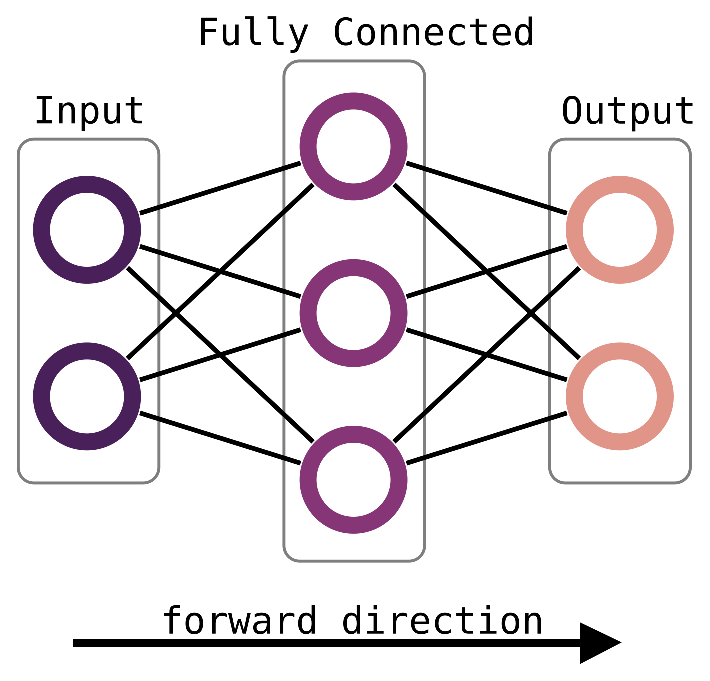
\includegraphics[width=0.30\textwidth]{./4_nn/figs/nn_theory_fc.eps}
  \caption{Basic fully connected layer with 3 nodes, receiving connections from 2 input nodes and outputing connections to 2 output nodes.}
  \label{fig:nn_theory_fc}
\end{figure}
\FloatBarrier
\noindent
In one node usually following computation is processed:
\begin{equation}
  z = h(w \, x^T + b)
\end{equation}
with the same notations as in \req{nn_theory_acti} and an additional bias term $b \in \R$.


% --
% cnn

\subsection{Convolutional Layers}\label{sec:nn_theory_cnn}
Convolutional layers are the fundament of every Covolutional Neural Networks (CNN) as already discussed in \rsec{prev_nn_cnn}.
They use convolutional filters on small areas of the input data, so that spatial information is retrieved.
Those convolutional filters are also called kernels and illustrated in case of images as rectangle in 2D space with kernel width $k_w$ and height $k_h$.
The kernel is shifted over its input map in each axis with an operation called \emph{stride}, denoted as $s$, and produce a output map through convolution.
The output dimension $o_d$ for striding along this axis with $s_d$ and kernel size for that axis $k_d$ over the input dimension $i_d$ can be computed as:
\begin{equation}\label{eq:nn_theory_cnn_}
  o_d = \floor*{\frac{i_d + p_d - k_d}{s_d} + 1}
\end{equation}
where $p_d$ is additionally a \emph{padding} term, where for instance for in zero-padding, zeros are added on both sides of the input dimension.
For example if a $16 \times 16$ image is convoluted by a $5 \times 5$ kernel with stride $1$ in each direction and no padding, the output image is $12 \times 12$.
The padding operation has usually the purpose to keep a the output and input dimension the same.
This is used for instance in residual neural networks, where the input to convolutional layers of a block, is bypassed and added to the output of this block again.
Being able to compute the addition operation from input and output of the residual block, their dimensions must be the same.
However in most convolutional network applications without residual blocks, it is preferred not to pad the image, so that dimensions are reduced hence parameters and multiplications saved.
Further there exist some special convolutional layers designed to reduce the dimensions (subsampling), such as a Max-Pooling layer. 

As already mentioned above CNNs are defined with the amount of input and output channels (feature maps), the kernel size, the stride of the kernel and some other specialties like dilation.
However it is not immediately clear from those parameter, how many convolutional filters are applied and what how the output feature maps are calculated exactly.
The amount of convolutional filters is in most practical examples always:
\begin{equation}\label{eq:nn_theory_n_filters}
  \#k = i \cdot j
\end{equation}
where $i$ and $j$ is the amount of input and output channels respectively.
Each kernel produces an output map, but the idea is to constraint the number of output maps $\#k$ to the defined output channels $j$.
This is usually done by summing up all output maps of input channels $i$ for one output channel $j$:
\begin{equation}
  o_j = \sum_{i} k_{i, j} * x_i
\end{equation}
where $o_j$ is the j-th feature map, $k_{i, j}$ the kernel of $i$ and $j$ and $x_i$ the i-th input channel.
A gaphical example of this procedure is shown in \rfig{nn_theory_cnn_basics}.
% cnn basics
\begin{figure}[!ht]
  \centering
    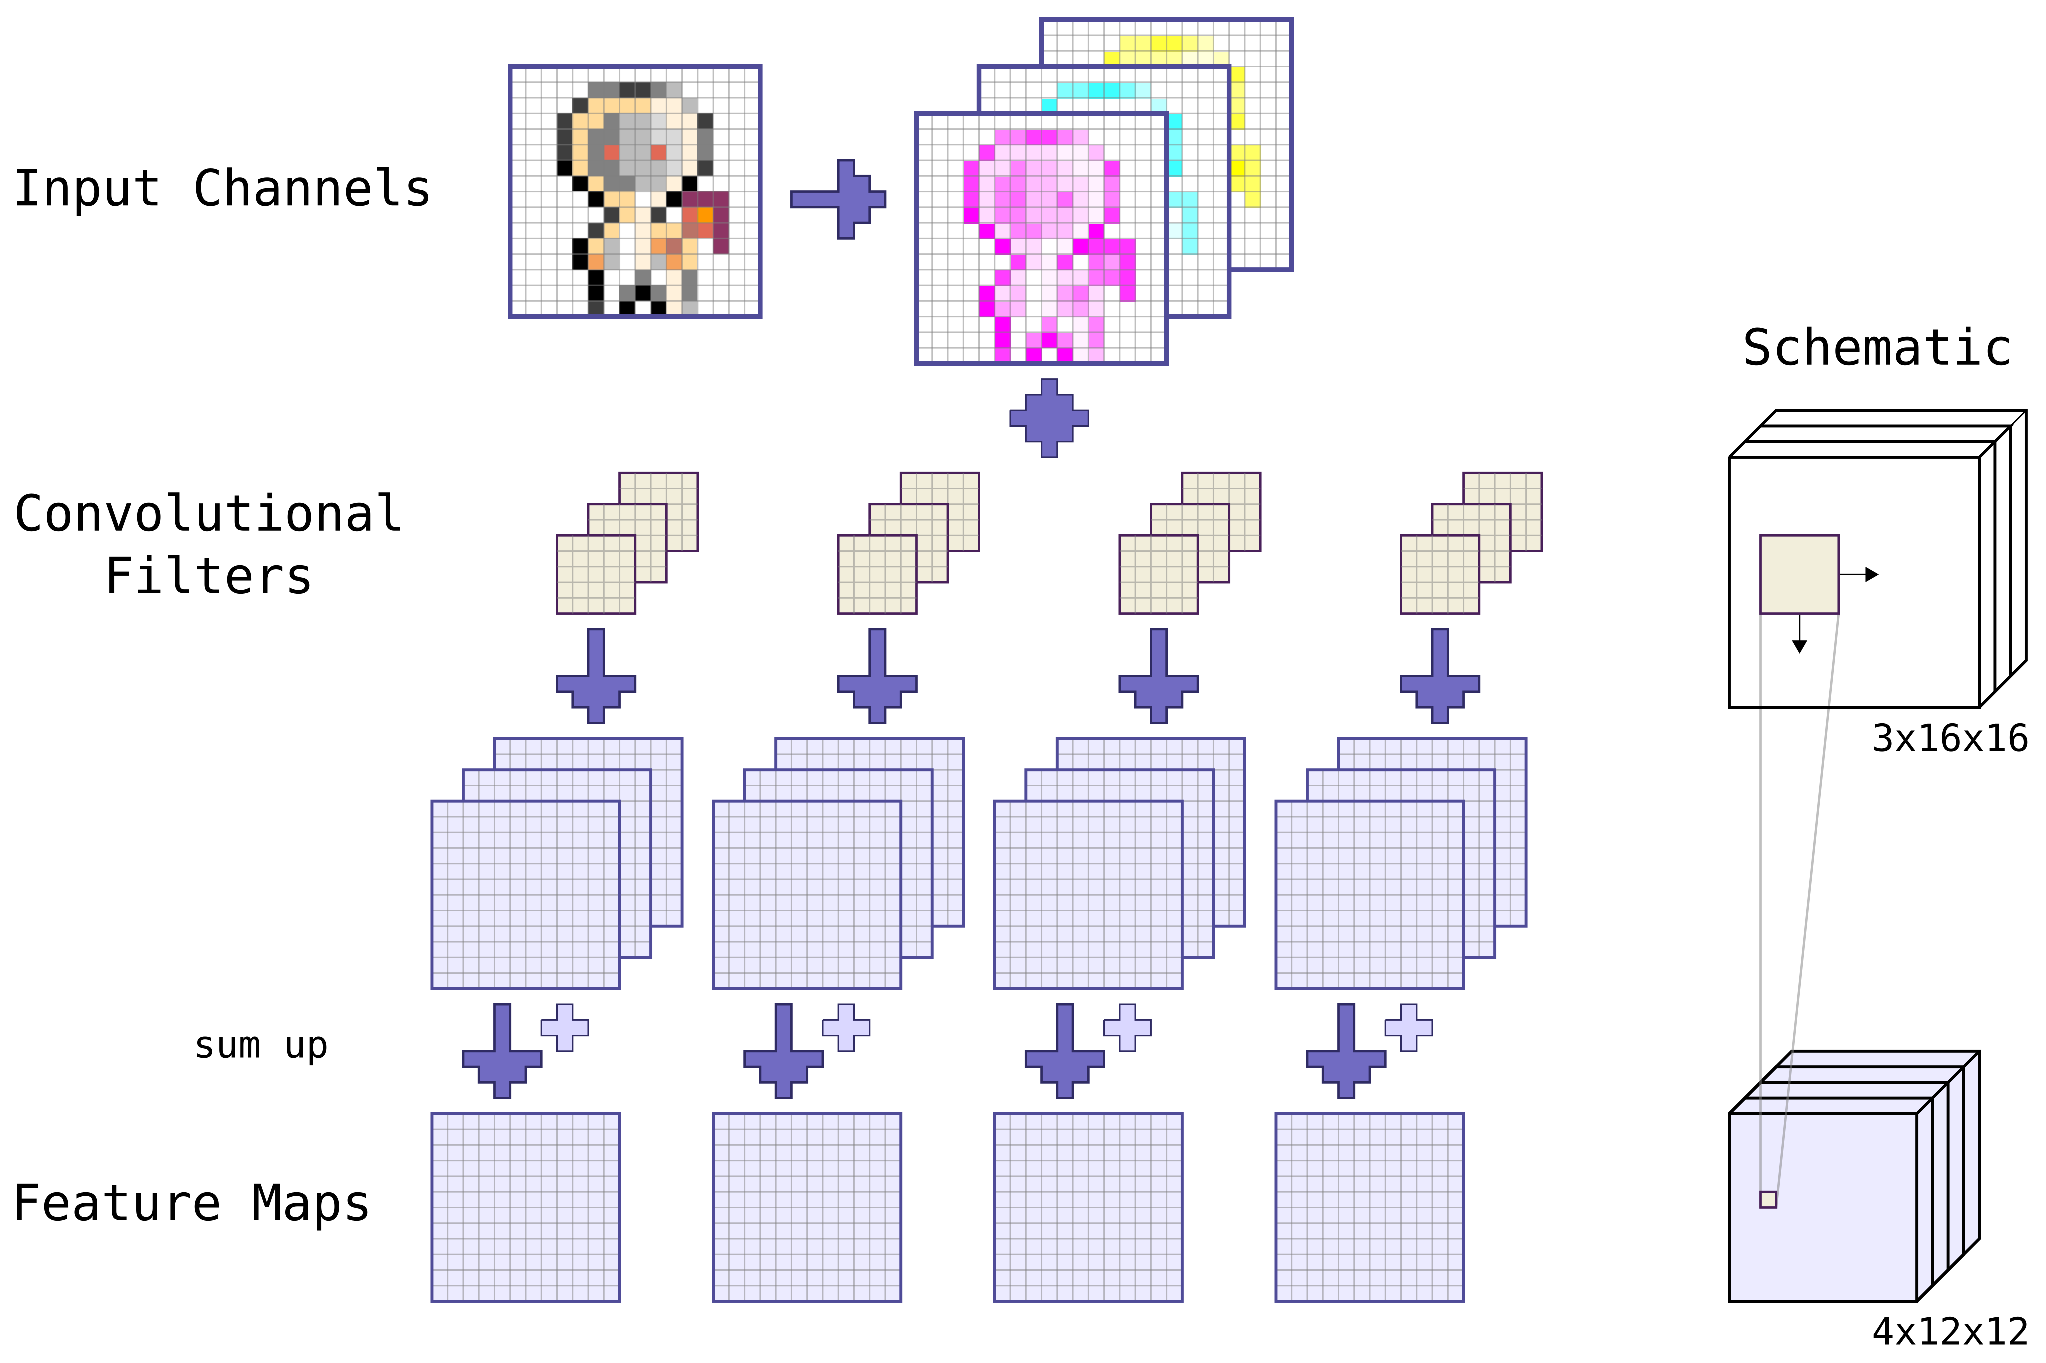
\includegraphics[width=0.6\textwidth]{./4_nn/figs/nn_theory_cnn_basics.eps}
  \caption{Basic CNN layer with a $16 \times 16$ input image, decomposed in 3 channels (CYM) and 4 output feature maps. Kernel size is $5 \times 5$ and the stride is $1$.}
  \label{fig:nn_theory_cnn_basics}
\end{figure}
\FloatBarrier
\noindent


% --
% loss functions

\subsection{Loss Functions and Softmax}
Loss functions or also called cost functions are used to calculate the difference between the predicted labels $\hat{y}$ compared to the actual or ground truth labels $y$.
The predicted labels are usually presented by the output nodes in the last layer of a neural network.
Therefore $\hat{y} = [\hat{y_1}, \, \hat{y_2}, \dots, \hat{y_c}]^T$ has the dimension of the number of labels or classes $c$.
Often it is preferred that $\hat{y} \in R^c$ provides a probability distribution such that:
\begin{equation}
  \sum_{i=0}^c \hat{y}_i = 1
\end{equation}
which can be achieved with the softmax function:
\begin{equation}\label{eq:nn_theory_softmax}
  \hat{y}_i = \frac{\exp{x_i}}{\sum_{j=0}^{c}\exp{x_j}}
\end{equation}
where $c$ is the amount of nodes in this layer, if it is the last layer as usual for the softmax, $c$ is the amount of classes and $\hat{y}_i$ the probability value of the corresponding class $i$.


% --
% dropout

\subsection{Dropout}
Dropout is a method to improve generalization and training of neural network.
The idea is to set the output of randomly selected nodes within a layer and for one training step to zero, so that only the other nodes are updated.
This can be simply done by multiplying all outputs of a current layer with a vector containing a number of zeros and ones places at random positions within the vector.
The amount of zeros compared to ones can be determined by a probability value, for instance $p=0.2$ means that there are 20\% zeros and 80\% ones within the vector.


% --
% training

\subsection{Training of a Neural Network}
The training process of a neural network is usually done with backpropagation of gradients from a loss function at the output nodes.
The backpropagation algorithm is not described here, because there exists many books and papers such as ... with good formulations, further it does not add any value to this thesis as the algorithm is run in the background of all neural network frameworks.
The interesting elements are therefore only the neural network architecture and the loss functions.


% architectures
% --
% Neural Network Architectures

\section{Neural Network Architectures}\label{sec:nn_arch}
All neural network Architectures evaluated within this thesis are presented here.
In general the used architectures were:
\begin{enumerate}
	\item Convolutional Neural Networks (CNN)
	\item Generative Adversarial Neural Networks (GAN)
	\item Wavenets
\end{enumerate}
The term convolutional neural network here consists of all architectures consisting of at least one convolutional layer and the intention to simply classify each speech commands from each other. 
Therefore the output of a convolutional net is of size of the number of individual speech commands and usually has some kind of probability distribution or energy equivalence.

With adversarial neural networks all architectures are meant, with at least two separate neural network Architectures, e.g. a Discriminator and a Generator Network and the intention to outperform the other Network in a task where both play a game against each other.
The word game is meant in the sense of game theory, where the goal is to find an equilibrium state of players competing against each other.
An equilibrium state is usually found if all players are satisfied with the outcome.
In this thesis the amount of players, or neural networks, is always two.
An overview of all models is shown in \rtab{nn_arch_overview} with abbreviations in \rtab{nn_arch_abbreviation}.
\begin{table}[ht!]
\small
\begin{center}
\caption{Network Architectures Abbreviations}
\begin{tabular}{ M{2.5cm}  M{10cm} }
\toprule
\textbf{Abbreviations} & \textbf{Meaning}\\
\midrule
c[0-9] & convolutional layer with layer number\\
f[0-9] & feed forward fully-connected layer with layer number\\
m[0-9] & max pooling layer layer with layer number\\
ch & input channel number for mfccs it is usually 1\\
fs & frame size (usually 50 -> 50ms)\\
ms & feature size (mfcc), depends on feature selection\\
cf & output number of last flattened convolutional layer\\
cl & number of class labels\\
\bottomrule
\label{tab:nn_arch_abbreviation}
\end{tabular}
\end{center}
\vspace{-4mm}
\end{table}
\FloatBarrier
\noindent
\begin{table}[ht!]
\begin{center}
\caption{Network Architectures Overview with reference names}
\begin{tabular}{ M{2.5cm}  M{2.1cm}  M{2.1cm} M{2.1cm} M{2.5cm}}
\toprule
%\multicolumn{4}{c}{\textbf{Feature Groups}} & \multicolumn{2}{c}{\textbf{Accuracy}} \\
\textbf{Reference name} & \textbf{Feature maps} & \textbf{Kernel sizes} & \textbf{Strides} & \textbf{Feed Forward} \\
\midrule
conv-trad & c1: (ch, 64) c2: (64, 64) & c1: (4, 20) mp: (2, 4) c2: (2, 4) & c1: (1, 1) mp: (2, 4) c2: (1, 1) & f1: (cf, 32) \quad f2: (32, 128) f3: (128, cl)\\
\midrule
conv-fstride & c1: (ch, 54) & c1: (8, fs) & c1: (4, 1) & f1: (cf, 32) \quad f2: (32, 128) \quad f3: (128, 128) \quad f4: (128, cl)\\
\midrule
conv-encoder-fc1 & c1: (ch, 48) \quad c2: (48, 8) & c1: (ms, 20) \quad c2: (1, 5) & c1: (1, 1) \quad c2: (1, 1) & f1: (cf, cl)\\
\midrule
conv-encoder-fc3 & c1: (ch, 48) \quad c2: (48, 8) & c1: (ms, 20) \quad c2: (1, 5) & c1: (1, 1) \quad c2: (1, 1) & f1: (cf, 64) \quad f2: (64, 32) \quad f3: (32, l)\\
\bottomrule
\label{tab:nn_arch_overview}
\end{tabular}
\end{center}
\end{table}
\FloatBarrier
\noindent



% adversarial
% --
% adversarial

\section{Adversarial Pre-Training}\label{sec:nn_adv}
\thesisStateRevised
In adversarial neural network training, two separate neural networks are competing against each other in an adversary task.
This competition of the two networks motivates them to improve their performance and beat the other network.
The application of GANs, as already explained in \rsec{prev_nn_adv} and \rsec{nn_theory_gan}, is an interesting subject in research and the questions whether the obtained weights from the training of the Generator (G) and Discriminator (D) network can contribute to better the performances in equivalent models, arises.
In the following the training algorithms are explained in more detail, such as the loss functions used for G and D.
The transfer of weights can be done for training instances on small subsets of labels or the whole network by regarding all labels at once in a single training instance.
%The transferring technique of the whole network is denoted as adversarial dual train and the training of separate labels is named adversarial label train.
The transferring technique of training instances on small subsets of labels is denoted as adversarial label train and the transfer of weights from a whole network with all labels is named as adversarial dual train.
In the following those training techniques are further explained, except of the adversarial dual train, because it is straight forward if the adversarial label train is explained.

% --
% training GANs

\subsection{Training Generative Adversarial Neural Networks}
The interesting part in training GANs is how the Generator (G) and Discriminator (D) models are updated in each training step and which loss functions were used.
In \req{nn_theory_gan} the game is notated as min-max game, from which the loss of D $l_D$ can be described for one specific training example $i$ of a batch as:
\begin{equation}
  l_D(x_i, z_i, G) = l(D(x_i), y_r) + l(D(G(z_i)), y_f)
\end{equation}
where $l$ is the binary cross-entropy loss described in \req{nn_theory_binary_cross_entropy}, $D: \mathcal{X} \mapsto [0, 1]$ and $G: \mathcal{Z} \mapsto \mathcal{X}$, $x_i \in \mathcal{X}$ is the data example, $z_i \in \mathcal{Z}$ is a randomly sampled latent variable, $y_r = 1$ is the real label and $y_f = 0$ the fake label for that specific example $i$.
In contrast the loss of the Generators $l_G$ is:
\begin{equation}
  l_G(z_i, D) =  l(D(G(z_i)), y_r)
\end{equation}
with $y_r$ as real label to perform maximization of $\log D(G(\bm{z}))$ as described in \rsec{nn_theory_gan}.
An extended approach, so that G produces samples specifically similar to the data distribution and does not drift off into creating unrealistic fakes of noisy samples to fake D, is to incorporate a similarity term with the \emph{cosine similarity}:
\begin{equation}
  s(\bm{x_1}, \bm{x_2}) = \frac{\bm{x_1}^T \bm{x_2}}{\norm{\bm{x_1}}_2 \cdot \norm{\bm{x_2}}_2 + \epsilon} 
\end{equation}
where $s : (\mathcal{X}, \mathcal{X}) \mapsto [0, 1]$ is the cosine similarity function, $\bm{x_1}$ and $\bm{x_2}$ are two vectors for similarity measure and $\epsilon$ is a small number, such that no division by zero is possible.
With the similarity loss incorporated, $l_G$ gets:
\begin{equation}
  %l_G(x_i, z_i, D) =  l(D(G(z_i)), y_r) + \lambda (1 - \E \left[ s(x_i \bm{e}, G(z_i)) \right])
  l_G(x_i, z_i, D) =  l(D(G(z_i)), y_r) + \lambda \left(1 - \frac{1}{C} \sum_{c=0}^{C} s(\hat{\bm{e}}_c^T x_i , \hat{\bm{e}}_c^T G(z_i)) \right)
\end{equation}
where $\hat{\bm{e}}_c \in \{1, 0\}^C$ is a unit vector representing one cepstral coefficient of the Mel Frequency Cepstral Coefficient (MFCC) data $x_i \in \mathcal{X} = \R^{C \times M}$ with a total number of $C$ MFCC coefficients and $M$ frames.
Further $\lambda$ is a trade-off factor between data similarity and fake loss from D.
For the experiments in \rsec{exp_adv}, $\lambda = 5$ was chosen.

The update of D and G can be done for each training step by backpropagating the obtained losses.
However it is more appealing if D is updated for a certain numbers of training steps with no update of G and then alternating to updates of G without updating D.
This will give either D or G some update steps to improve in their specific adversarial task of either discriminating or generating.
In this thesis the training steps for updating either D or G was selected to 2 epochs.
Note that an epoch consists of several training steps depending on the batch size and amount of data, this can vary for the experiments, however it does not influence that much on the overall end results.


% --
% label train

\subsection{Adversarial Label Train}
Adversarial label train, is the transfer of weights from feature maps trained on multiple GAN training instances on subsets of all labels.
For instance if the total amount of labels are \{\enquote{left}, \enquote{right}\} then an own training instance can focus on the label \enquote{left} and another on the label \enquote{right}.
It is important to assign a specific number of feature maps to each label train instance, for example each label train gets 8 feature maps of the first convolutional layers.
The label train scheme is illustrated in \rfig{nn_adv_label_scheme} and applies 6 label train instances, such as used for the experiments in \rsec{exp_adv}.
\begin{figure}[!ht]
  \centering
    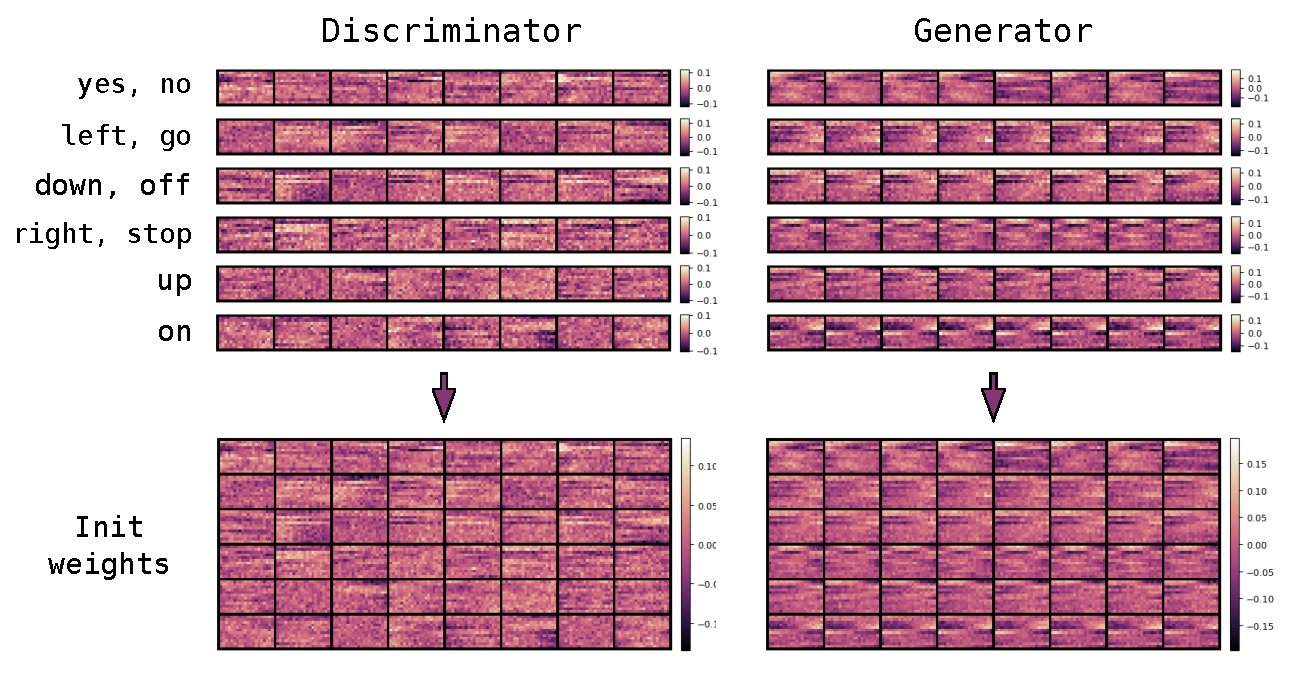
\includegraphics[width=0.7\textwidth]{./4_nn/figs/nn_adv_label_scheme}
  \caption{Label train scheme of 6 training instances, trained with 100 epochs for each label subset.}
  \label{fig:nn_adv_label_scheme}
\end{figure}
\FloatBarrier
\noindent
An actual GAN training for the labels \enquote{left} and \enquote{go} is shown in \rfig{nn_adv_loss_label}.
Note that the update of either the Discriminator (D) or Generator (G) model is done alternating for 2 training epochs.
\begin{figure}[!ht]
  \centering
  \subfigure[it-100]{\includegraphics[width=0.45\textwidth]{./4_nn/figs/nn_adv_loss_label_it-100}}
  \subfigure[it-1000]{\includegraphics[width=0.45\textwidth]{./4_nn/figs/nn_adv_loss_label_it-1000}}
  \caption{Adversarial training loss of the labels \enquote{left} and \enquote{go} with 8 feature maps.}
  \label{fig:nn_adv_loss_label}
\end{figure}
\FloatBarrier
\noindent
The creation of fake images from G is shown in \rfig{nn_adv_fakes_label} of the same training instances.
\begin{figure}[!ht]
  \centering
  \subfigure[it-100]{\includegraphics[width=0.45\textwidth]{./4_nn/figs/nn_adv_fakes_label_it-100}}
  \subfigure[it-1000]{\includegraphics[width=0.45\textwidth]{./4_nn/figs/nn_adv_fakes_label_it-1000}}
  \caption{Generation of fake images of the labels \enquote{left} and \enquote{go} with 8 feature maps for the GAN training.}
  \label{fig:nn_adv_fakes_label}
\end{figure}
\FloatBarrier
\noindent

As showcase example, some concatenated adversarial label train weights used for weight transfer, are shown for D and G with different amounts of training epochs in \rfig{nn_adv_label_weights_d} and \rfig{nn_adv_label_weights_g}.
\begin{figure}[!ht]
  \centering
  \subfigure[d-100]{\includegraphics[width=0.45\textwidth]{./4_nn/figs/nn_adv_label_weights_d-100}}
  \subfigure[d-1000]{\includegraphics[width=0.45\textwidth]{./4_nn/figs/nn_adv_label_weights_d-1000}}
  \caption{Concatenated label weights of the first convolutional layer from the Discriminator model with different amounts of epochs.}
  \label{fig:nn_adv_label_weights_d}
\end{figure}
\FloatBarrier
\noindent
\begin{figure}[!ht]
  \centering
  \subfigure[g-100]{\includegraphics[width=0.45\textwidth]{./4_nn/figs/nn_adv_label_weights_g-100}}
  \subfigure[g-1000]{\includegraphics[width=0.45\textwidth]{./4_nn/figs/nn_adv_label_weights_g-1000}}
  \caption{Concatenated label weights of the first convolutional layer from the Generator model with different amounts of epochs.}
  \label{fig:nn_adv_label_weights_g}
\end{figure}
\FloatBarrier
\noindent
The amounts of epochs are important, because they determine how much the models are learning in their adversarial task.
With 100 epochs the Generator creates similar feature maps for each label train instance, because it does not need to be that accurate in creating different looking fakes, however the Discriminator gets better as well and the need of generating different looking fakes are necessary to match up.
With 1000 epochs the Generator produces already different fakes as already shown in \rfig{nn_adv_fakes_label} however it is not recommended to train for too long.
Note that a second convolutional layer for the \texttt{adv-d-jim} and \texttt{adv-g-jim} exist as well, the corresponding weights are shown only for the 100 epoch examples in \rfig{nn_adv_label_weights_conv1}.
\begin{figure}[!ht]
  \centering
  \subfigure[d-100]{\includegraphics[width=0.25\textwidth]{./4_nn/figs/nn_adv_label_weights_conv1_d-100}}
  \qquad \qquad
  \subfigure[g-100]{\includegraphics[width=0.25\textwidth]{./4_nn/figs/nn_adv_label_weights_conv1_g-100}}
  \caption{Concatenated label weights of the second convolutional layer from the Discriminator and Generator model with trained with 100 epochs.}
  \label{fig:nn_adv_label_weights_conv1}
\end{figure}
\FloatBarrier
\noindent
From the second convolutional layer each row corresponds to a single feature map and therefore 8 rows to one adversarial label training instance.
% \subsection{Questions that arise}
% There are several questions that arise regarding Adversarial Training:
% \begin{enumerate}[label={Q.\textgoth{A}.\arabic*)}, leftmargin=1.4cm]
%   \item Does the Network Architecture of G and D have to be the same but transposed?
%   \item Does the value space of in and outputs, for D and G respectively, have to be limited between a range of [0, 1] done by for instance the frame normalization, or sigmoid output?
%   \item What loss function works well for training?
%   \item How long should be trained?
%   \item When transfering weights to another network, should the weights from G or D be transfered?
%   \item Does the classification network has to adapt the parameters from the transfered weights?
%   \item Whats the benefit of all this?
% \end{enumerate}

% To illustrate the idea an example is shown of the labels L5 (left, right, up, down, go).

% The convolutional layer weights from the adversarial training of the individual labels, 
% can be stacked together an used to initialize another network.
% An example of this method is shown in \rfig{nn_adv_example}, where the initialization pattern changes to more elaborate structures and patterns to form good classification outputs. 
% However the Basic Pattern from the adversarial training stays the same, which is a good sign, because then the network is accepting those trained weights and adapts them.

% \begin{figure}[!ht]
%   \centering
%     \subfigure[c1 trained]{\includegraphics[width=0.45\textwidth]{./4_nn/figs/nn_adv_example_c0}}
%     \subfigure[c1 init]{\includegraphics[width=0.45\textwidth]{./4_nn/figs/nn_adv_example_c0_init}}
%     \subfigure[c2 trained]{\includegraphics[height=0.45\textwidth]{./4_nn/figs/nn_adv_example_c1}}
%     \quad
%     \subfigure[c2 init]{\includegraphics[height=0.45\textwidth]{./4_nn/figs/nn_adv_example_c1_init}}
%   \caption{Adversarial Training Example: Convolutional layers pretrained with adversarial training on each label separately.}
%   \label{fig:nn_adv_example}
% \end{figure}
% \FloatBarrier
% \noindent

% For this example in adversarial training, 8 feature maps of the first layer were used for each label, also they belong to the Generator Network G or decoder (dec). In Convolutional Networks, each previous layers feature map creates a new set of feature maps in the next layer.
% An example of this label training is shown in \rfig{nn_adv_example_label} with feature maps [(1, 8), (8, 8)] of the convolutional layers

% \begin{figure}[!ht]
%   \centering
%     \subfigure[\enquote{left} c1 from D]{\includegraphics[width=0.45\textwidth]{./4_nn/figs/nn_adv_example_label_left_c0_enc}}
%     \subfigure[\enquote{left} c1 from G]{\includegraphics[width=0.45\textwidth]{./4_nn/figs/nn_adv_example_label_left_c0_dec}}
%     \subfigure[\enquote{left} c2 from D]{\includegraphics[width=0.3\textwidth]{./4_nn/figs/nn_adv_example_label_left_c1_enc}}
%     \subfigure[\enquote{left} c2 from G]{\includegraphics[width=0.3\textwidth]{./4_nn/figs/nn_adv_example_label_left_c1_dec}}
%   \caption{Adversarial Training example of Generator (G) and Discriminator (D) of label \enquote{left} captured with 8 feature maps of the first convolutional layer.}
%   \label{fig:nn_adv_example_label}
% \end{figure}
% \FloatBarrier
% \noindent

% Those trained weights from each label can then simply be put into the feature maps of a classification network.
% This is shown in \rfig{nn_adv_example} where c1 from G and c2 from G in \rfig{nn_adv_example_label} were transfered to the first row(s).
% When doing the transferring of feature maps, it is important that the layers are not mixed up so that the trained connections are still correct.
% Also of course the weights of the feature maps must have the same dimension, so that transferring is possible.


% \subsection{Observing the Generators output}
% While the output of the Discriminator is rather uninteresting (one-dimensional probability value), the output of the Generator is a good indicator of how well the training between D and G has gone.
% Optimally the output of the Generator look like real data samples.
% An example of a trained Generator Network with fake outputs compared to real ones is shown in \rfig{nn_adv_gen}.

% \begin{figure}[!ht]
%   \centering
%     \subfigure[\enquote{left} real examples]{\includegraphics[width=0.45\textwidth]{./4_nn/figs/nn_adv_gen_left_real}}
%     \subfigure[\enquote{left} fakes from G]{\includegraphics[width=0.45\textwidth]{./4_nn/figs/nn_adv_gen_left_fake}}
%   \caption{Real samples of \enquote{left} from the Speech Commands dataset compared to fake samples from a trained Generator Network.}
%   \label{fig:nn_adv_gen}
% \end{figure}
% \FloatBarrier
% \noindent

% If the fake example of the Generator Network do not look similar to real ones, then something might have gone wrong in the training between the Generator and Discriminator Network.
% Further it can be evaluated if a certain network architecture is able to produce a label in a sufficient representation, therefore this method might be a good start in finding a suitable network architecture for the problem to be solved.




% --
% Experiments

\chapter{Experiments}\label{sec:exp}
All experiments hold within this thesis can be found in this chapter.
At the start it gives inside to the the Datasets and its feature extraction used for training the neural network architectures.
Some sound examples and their feature representation of the datasets are shown and the quality and diversity of recorded samples is mentioned.

More importantly this chapter includes the evaluation of the neural network models and their feature inputs in the application of speech command classification.
In Detail the feature selection is evaluated, to observe the impact of feature reduction.
Further the adversarial training approaches are compared to usual training.
Then the wavenet performances are shown...

% The training details are listed to give the reader an overview of the selected parameters for training, it should also give a shorten reference, so that not all parameters must be listed in the plots. 
% The training and evaluation consists of following evaluation tasks:
% \begin{enumerate}
%   \item Feature Selection
%   \item Adversarial Training
% \end{enumerate}

% dataset
% --
% dataset

\section{Dataset}\label{sec:exp_dataset}
\thesisStateReady
Two datasets are used within this thesis, one is the second version of the speech commands dataset from \cite{Warden2018} and one is self made, denoted as \enquote{my dataset} which consists of only 5 labels that are especially valuable for movement in video games.
Note that the \enquote{my dataset} is merely used for evaluation.
The training, validation and testing of the neural network architectures is done on the speech commands dataset.
Both datasets consists of raw waveform files in the \texttt{.wav} format, no feature extraction was done beforehand.
As already mentioned in \rsec{prev_kws_benchmark} direct comparisons between different neural network approaches is difficult if the feature extraction is left to the user alone.
Some datasets provide feature extraction beforehand, so that the comparability of neural network architectures performances is not influenced on it.
The speech commands dataset does not explicitly separate each \texttt{.wav} file into train, test and validation sets, but provides file lists that refers to distinct waveform files that should be used for testing and validation and therefore gives a guidline for comparison.
More details of the datasets are presented below.

% Some abbreviations and references were done, so that the jungle of selected parameters get a little bit more clear to the reader of this thesis.in the \texttt{.wav} format
% The abbreviations of the dataset are shown in \rtab{exp_dataset_abbr}.

% The speech commands dataset is extracted before it is used for training. 
% To reduce computations in the evaluation process of neural networks, it was important to reduce the number of classes and examples per class to an suitable number.

% \input{./5_exp/tables/tab_exp_dataset_abbr.tex}


% --
% speech commands dataset

\subsection{Speech Commands Dataset}\label{sec:exp_dataset_speech_cmd}
The speech command dataset \cite{Warden2018} exists in two versions (\texttt{v0.01} and \texttt{v0.02}), the first one was published in 2017 and the second one emerged as improved version of \texttt{v0.01} with 5 more key words \{\enquote{backward}, \enquote{forward}, \enquote{follow}, \enquote{learn}, \enquote{visual}\}, class examples and quality in 2018.
The  dataset consists of \SI{1}{\second} speech recordings of 30 different words in \texttt{v0.01} and 35 different words in \texttt{v0.02}, done by over thousands of individual speakers.

In this thesis, the experiments are done on the second version \texttt{v0.02} of the dataset.
The hard-facts about the speech command dataset \texttt{v0.02} are listed in \rtab{exp_dataset_hard_facts}.
% hard facts
\begin{table}[ht!]
\begin{center}
\caption{Hard facts of the speech commands dataset \texttt{v0.02}.}
\begin{tabular}{ M{5cm}  M{2cm} }
\toprule
%\textbf{label} & \textbf{train} \\
%\midrule
Total number of key words & 35\\
Total number of examples & 105886\\
Total number of speakers & 2618\\
\midrule
%Number of core key words & 20\\
%Number of auxiliary key words & 15\\
Recording duration & 0.4 - \SI{1}{\second}\\
Channels & Mono\\
Bit depth of audio files & \SI{32}{\bit}\\
Sampling frequency & \SI{16}{\kilo\hertz}\\
\bottomrule
\label{tab:exp_dataset_hard_facts}
\end{tabular}
\end{center}
\end{table}
\FloatBarrier
\noindent


All speech command key words with their separation in training, test and validation set are shown in \rtab{exp_dataset_all_labels}.
% all labels tab
\begin{table}[ht!]
\small
\begin{center}
\caption{All labels and counts of available data examples for each set obtained from the speech commands dataset \texttt{v0.02}.}
\begin{tabular}{ M{2cm}  M{1.75cm}  M{1.75cm}  M{1.75cm}  M{1.75cm} }
\toprule
\textbf{label} & \textbf{train} & \textbf{test} & \textbf{validation} & \textbf{total} \\
\midrule
backward & 1346 & 165 & 153 & 1664 \\
bed & 1624 & 234 & 213 & 2071 \\
bird & 1697 & 185 & 182 & 2064 \\
cat & 1657 & 194 & 180 & 2031 \\
dog & 1711 & 220 & 197 & 2128 \\
down & 3134 & 406 & 377 & 3917 \\
eight & 3033 & 408 & 346 & 3787 \\
five & 3240 & 445 & 367 & 4052 \\
follow & 1275 & 172 & 132 & 1579 \\
forward & 1256 & 155 & 146 & 1557 \\
four & 2955 & 400 & 373 & 3728 \\
go & 3106 & 402 & 372 & 3880 \\
happy & 1632 & 203 & 219 & 2054 \\
house & 1727 & 191 & 195 & 2113 \\
learn & 1286 & 161 & 128 & 1575 \\
left & 3037 & 412 & 352 & 3801 \\
marvin & 1710 & 195 & 195 & 2100 \\
nine & 3170 & 408 & 356 & 3934 \\
no & 3130 & 405 & 406 & 3941 \\
off & 2970 & 402 & 373 & 3745 \\
on & 3086 & 396 & 363 & 3845 \\
one & 3140 & 399 & 351 & 3890 \\
right & 3019 & 396 & 363 & 3778 \\
seven & 3205 & 406 & 387 & 3998 \\
sheila & 1606 & 212 & 204 & 2022 \\
six & 3088 & 394 & 378 & 3860 \\
stop & 3111 & 411 & 350 & 3872 \\
three & 2966 & 405 & 356 & 3727 \\
tree & 1407 & 193 & 159 & 1759 \\
two & 3111 & 424 & 345 & 3880 \\
up & 2948 & 425 & 350 & 3723 \\
visual & 1288 & 165 & 139 & 1592 \\
wow & 1724 & 206 & 193 & 2123 \\
yes & 3228 & 419 & 397 & 4044 \\
zero & 3250 & 418 & 384 & 4052 \\
\_noise\footnotemark & 2863 & 357 & 357 & 3577 \\
\bottomrule
\label{tab:exp_dataset_all_labels}
\end{tabular}
\end{center}
\vspace{-4mm}
\end{table}
\FloatBarrier
\noindent
\footnotetext{The noise label was added from the provided noise files, as described in \rsec{exp_dataset_structure}.}
In \rtab{exp_dataset_all_labels} it can be observed, that some labels are occurring significantly more often than others.
The idea behind this is, as described in \cite{Warden2018}, to separate the key words into \emph{core key words} and \emph{auxiliary key words}.
The core key words are the more frequent ones with about 3000 to 4000 examples each, in detail they are \{\enquote{yes}, \enquote{no}, \enquote{up}, \enquote{down}, \enquote{left}, \enquote{right}, \enquote{on}, \enquote{off}, \enquote{stop}, \enquote{go}, \enquote{zero}, \enquote{one}, ..., \enquote{nine} \}.

The auxiliary words are the less frequent ones that are not already listed above in the core key words of all available key words in the dataset.
The intention is that the core key words should be classified individually and therefore get an own class label each. 
The auxiliary key words should gather to a single separate class label representing all other possible unknown words to the classification system.
Those auxiliary key words are often labeled in papers with \enquote{unknown}, but in this thesis it is referred as \enquote{\_mixed} label.
Further some of the auxiliary key words are similar to core key words, such as \enquote{three} and \enquote{tree}, which should increase the difficulty in the classification task. 
In the creation of the examples for the \enquote{\_mixed} label, it is important to have an equal amounts of examples per individual auxiliary key word.

Some examples of the speech command dataset in raw audio format are shown in \rfig{exp_dataset_wav_grid_speech_commands_v2} to provide a small glimpse on the recordings.
\begin{figure}[!ht]
  \centering
    \includegraphics[width=0.65\textwidth]{./5_exp/figs/exp_dataset_wav_grid_speech_commands_v2}
  \caption{One random sample of each individual speech command in the speech command dataset in normalized raw audio format.}
  \label{fig:exp_dataset_wav_grid_speech_commands_v2}
\end{figure}
\FloatBarrier
\noindent


% --
% statistics

\subsubsection{Observations of all examples in the dataset}
Two histograms were created to observe the quality of all recorded files, those are an energy measure for each file and the count of the sample length.
The energy of a recorded file provides information about if a recording is too silent (background noise only) or too loud (overdrive distortions). In the first version of the speech command dataset (\texttt{v0.01}) too silent files were an issue.
Luckily this was solved in the second version by rejecting those silent files.
The energy value $e \in \R$ is computed as:
\begin{equation}\label{eq:exp_dataset_energy}
  e = \frac{1}{n} \left( x\, x^T \right)
\end{equation}
where $x \in \R^n$ are the values of all samples from the recorded files.
The division through the length each individual file in samples $n$, has to be done, because not every file has a \SI{1}{\second} duration with 16000 samples.
The sample length is simply the amount of samples in a recording file, those ideally should have a duration of \SI{1}{\second}, but for some unknown reason some of the recordings have less.
It would be problematic if the sample length is too low to capture a word, but the minimum duration of all files is about \SI{0.4}{\second}, and this is enough for words like \enquote{go}, etc.
The histograms of all available examples in the dataset are shown in \rfig{exp_dataset_hist}.

\begin{figure}[!ht]
  \centering
    \subfigure[energy]{\includegraphics[width=0.45\textwidth]{./5_exp/figs/exp_dataset_hist_energy_overall}}
    \subfigure[sample length]{\includegraphics[width=0.45\textwidth]{./5_exp/figs/exp_dataset_hist_sample_overall}}
  \caption{Energy value and sample length histograms in log-log and log-scale respectively of all examples in the speech commands dataset \texttt{v0.02}.}
  \label{fig:exp_dataset_hist}
\end{figure}
\FloatBarrier
\noindent
The energy histogram has one main lobe, which is good, so it means that there are no clusters of extremely silent or loud files.
For comparison, if silent files were extracted from for instance the given background files, the energy of some of those is in range of $10^{-7} \dots 10^{-6}$. Therefore it seems that most of the files are okay.
The sample length histogram shows, that most of the files have a duration of \SI{1}{\second}, but many other have less sample numbers. 
This is important and has to be regarded in the pre-processing of audio files, because the neural networks inputs are usually a fixed size input, if no sequential neural networks are deployed, such as Recurrent Neural Networks (RNN).


% --
% recording quality

\subsubsection{Recording Quality and Personal Experience}
The examples within the dataset were not recorded by professionals with high-end recording equipment, in fact the recordings had been done in an amateur kind of fashion, so that the dataset is more suited to realistic environments intended for user applications.
This is also noted in the paper \cite{Warden2018}:
\begin{quote}
...This meant that the use of studio-captured samples seemed unrealistic, since that audio would lack background noise, would be captured with high-quality microphones, and in a formal setting. 
Successful models would need to cope with noisy environments, poor quality recording equipment, and people talking in a natural, chatty way...
\end{quote}
The recording devices of the speakers, who contributed examples to the dataset, were in most cases simple consumer microphones, as for instance deployed in laptops or mobile phones.

The personal experiments made, when listening to the examples in the dataset, were:
\begin{itemize}
  \item The quality of the examples in the dataset are ranging from really good and understandable to very bad, noisy, unrecognizable and cut away, though most of the examples are good.

  \item Different accents can be perceived, that suggests that people from several countries were involved. However the bias is layed on American English as noted in the paper.

  \item No children speakers were found on the personal listening.
\end{itemize}

Due to data privacy issues the information on the individual speakers are not given.
Further it is not clear if there are equal amounts of male and female speakers and if there are any children speakers included.
The last would be especially interesting for a video games suited for kids.

In many recordings the background noise is imminent, such as traffic noise, chattering people, office sounds, etc.
A quality check of the recorded files in the dataset was done, as described in \cite{Warden2018}, to ensure that bad samples are rejected.
However there are still some existing flaws such as extremely loud or silent files or examples with inconsistent sample numbers or too much noise in it or in the worst case, noise only (very rarely).
Those quality issues in the dataset are for most cases neglectable or can be fixed, such as inconsistent sample numbers. 
Other more problematic cases, for instance noise-only examples, should actually be filtered out, but since their occurrence is very rare, it is not worth the effort.
%Still it is a great dataset, because there is no need for a perfect dataset when working with neural networks and one can be happy that there exists one with this amount of diversity and free of access under the creative common license.
Usually it is not a problem for neural networks to cope with noisy datasets, actually it is good if many noisy samples are contained, so that they could learn invariance against noise, loudness differences and other nuisances during training.
Further if the training dataset is large enough and the test and validation sets do not contain very bad examples, there should be no problem in training and evaluation of different models.


% --
% dataset structure

\subsubsection{Dataset Structure}
The speech command examples are stored in separate folders named after each individual key word, in the \texttt{.wav} format.
The folder named as \texttt{\_background\_noise\_} contains six different background noise files, such as \texttt{white\_noise.wav} or \texttt{doing\_the\_dishes.wav}, with a duration of more than one minute each.
Noise examples with a new noise label named \texttt{\_noise} were extracted from those background noise files with a \SI{1}{\second} window shifted by \SI{0.2}{\second}.

Each waveform file is named with an 8-digit hexadecimal hash code for the speaker identification, followed by the utterance number, for instance \texttt{3b4f8f24\_nohash\_0.wav}.
Therefore it is possible to distinguish between different speakers, however as mentioned above, no further information about the speaker is given due to data privacy issues.

Further the dataset provides a testing file list called \texttt{testing\_list.txt} and a validation file list \texttt{validation\_list.txt} where each row entry refers to a file in the dataset, for example \texttt{right/bb05582b\_nohash\_3.wav}
Those file lists for testing and validation should ensure the comparability between different neural network approaches from individual researchers.
In this thesis, those file list are applied and the separation into the sets already shown in \rtab{exp_dataset_all_labels}.


% --
% my dataset

\subsection{My own Dataset}\label{sec:exp_dataset_my}
This dataset was created by the author of this thesis and contains five examples samples each from the words \{\enquote{left}, \enquote{right}, \enquote{up}, \enquote{down} and \enquote{go}\}.
The datasets purpose is mainly to have an additional test set for evaluating trained models on the authors own voice with different word pronouncement on each example.
It is important to mention that none of the self recorded files were used within the training set, so that the neural networks performance on this unseen data is evaluated.
All examples of my own dataset are illustrated in \rfig{exp_dataset_wav_grid_my} in raw audio format.
\begin{figure}[!ht]
  \centering
    \includegraphics[width=0.65\textwidth]{./5_exp/figs/exp_dataset_wav_grid_my}
  \caption{Self recorded files of the \enquote{my dataset} in raw audio format.}
  \label{fig:exp_dataset_wav_grid_my}
\end{figure}
\FloatBarrier
\noindent
The examples per word are spoken with different emphasis and stress on individual phonemes.
Also the prolongation of the words are different, that in one example the word is fast and in the other its slow spoken.
The emphasis and prolongation ensure the diversity of the dataset. 
It turned out that it is not easy for neural networks to gain a $100\%$ classification score upon it, even though there is only one and the same speaker.


% --
% preparation for neural networks

\subsection{Data preparation for neural networks}\label{sec:exp_data_prep}
The neural networks architectures are trained with supervised learning, that means a class label $y_i$ correspondence to each data example $x_i$ must exist.
Some selected examples and their labels form a dataset $S$ for example for training or testing and can be written as:
\begin{equation}\label{eq:exp_dataset}
  S = \{ (x_i, y_i) | i = 0 \dots n \}
\end{equation}
where $n$ is the total number of examples within the dataset.

It was already shown how to extract MFCC features in \rsec{signal_mfcc}, however it is important that each individual $x_i$ for all $i$ has the same dimension.
It could happen that the sample numbers of the waveform files are inconsistent as describe in \rsec{exp_dataset_speech_cmd} and therefore yield different dimension for different $x_i$.
To ensure that each $x_i$ has the same dimension, the audiofiles were adjusted to have the same sample length of a duration of \SI{1}{\second} with sampling frequency \SI{16}{\kilo\hertz}.
This was done by simply zero-padding the signals to the desired length of 16000 samples.
Further some dither noise was added, so that neural networks are not confused when seeing pure zeros emerging from the data examples.
The dithering is usually done by Gaussian additive noise as describes:
\begin{equation}\label{eq:exp_dither}
  x = \tilde{x} + v, \quad v = \mathcal{N}(\mu=0, \sigma=0.5) \cdot \tilde{x}_{quant}%, \quad \mu, \sigma = 0, 0.5
\end{equation}
where $\mathcal{N}$ is the normal distribution, $\tilde{x}$ the zero-padded signal (if the sample numbers were incorrect) and $\tilde{x}_{quant}$ the quantization error, corresponding to the minimal absolute value of all samples of $\tilde{x}$ except the pure zero entries.
When the dithering is applied to the signal, it has no pure zeros anymore and it is not altered much from the origin, since the maximum change lies in a normal range of the quantization noise from the original recording quantization.
%% --
% Speech Commands dataset

\subsection{Speech Commands Dataset}\label{sec:exp_dataset_speech_cmd}
The speech command dataset \cite{Warden2018} is a very diverse dataset consisting of over thousands of different speakers. 
This dataset is by any means no clean dataset recorded by professionals, if anything it is the opposite and therefore more suitable to realistic environments, as noted in the paper:
\begin{quote}
...I made the decision to focus on capturing audio that reflected the on-device trigger phrase task described above. 
This meant that the use of studio-captured samples seemed unrealistic, since that audio would lack background noise, would be captured with high-quality microphones, and in a formal setting...
\end{quote}
The recording devices of the speakers were simply the next microphones they could grab, such as in laptops or mobile phones.
In many recordings the background noise is imminent, such as traffic, chattering people, office sounds, etc.
Some quality check of the recorded files has been done to reject bad samples.
However there are still some existing flaws such as too loud or too silent files or examples with inconsistent sample numbers and some examples are prone with too much noise or in the worst case, noise only.
Those quality issues in the dataset are for most cases neglectable or can be fixed, such as inconsistent sample numbers, other more problematic cases, for instance noise only examples, should be filtered out.
%Still it is a great dataset, because there is no need for a perfect dataset when working with neural networks and one can be happy that there exists one with this amount of diversity and free of access under the creative common license.
Maybe its even better to have an unclean dataset, so that invariance against noise and loudness are learnt during training.

Some examples of the speech command dataset in raw audio format are shown in \rfig{exp_dataset_wav_grid_c30} and give a small inside on the quality of the recordings.
\begin{figure}[!ht]
  \centering
    \includegraphics[width=0.65\textwidth]{./5_exp/figs/exp_dataset_wav_grid_c30}
  \caption{One random sample of each individual speech command in the speech command dataset in normalized raw audio format.}
  \label{fig:exp_dataset_wav_grid_c30}
\end{figure}
\FloatBarrier
\noindent

%It has to be mentioned, that it is wonderful, that a dataset for simple key word spotting on speech commands with this amount of diversity and free of access under the creative common license exist.


%% --
% my dataset

\subsection{My own Dataset}\label{sec:exp_dataset_my}
The author of this thesis recorded some speech command samples by himself and used it as own test set in evaluating trained models in the machine learning part. No self recorded files are used within the training set, so that it can be shown that unseen voice characteristics are classified correctly.
All examples of my own dataset are illustrated in \rfig{exp_dataset_wav_grid_my} in raw audio format.

\begin{figure}[!ht]
  \centering
    \includegraphics[width=0.65\textwidth]{./5_exp/figs/exp_dataset_wav_grid_my}
  \caption{My wav grid}
  \label{fig:exp_dataset_wav_grid_my}
\end{figure}
\FloatBarrier
\noindent

% neural networks
% --
% training details

\section{Implementation and Experiment Details}\label{sec:exp_details}
\thesisStateReady
The implementation describes the used software tools for the experiments on the neural networks, such as the programming language and packages for the source code.
The training details provide commonly used sets of hyperparameters applied to train neural networks.
Note that the training details can vary between different experiments and models and that the listing provide merely an overview of all available parameters to choose from with recommendations of parameters for the speech command dataset.
If parameters are varying in some experiments, they are usually noted, otherwise the parameters listed were used.
The evaluation details of the models is described separately and evaluates the trained models upon accuracy and noise and shift invariance.


% --
% implementation notes

\subsection{Implementation Notes}\label{sec:exp_details_implementation}
The source code for this thesis was entirely written in \texttt{Python} with version $>3.8$ evaluated on a Linux operating system and is open source available at \cite{KWSGame}.
The operating system might be important if someone tries to run the python code on a \enquote{Windows} machine, where unexpected errors might occur (especially regarding path variables).
Also the project does not download the speech command dataset by its own and a path to the dataset has to be specified in the \texttt{config.yaml} file of the project.
More on information about how to run the project is described in the \texttt{README.txt} file.
The training and implementation of all used neural networks were done with the \texttt{Pytorch} \cite{Pytorch} framework of version $1.7.0$. 
Usually it should not be a problem if a newer version of \texttt{Pytorch} is used, during the work on the thesis the version changed to $1.9.0$ without any version depending problems.
The feature extraction of MFCCs was self implemented, but use already existing and efficient code for transforms, such as the STFT or DCT, with packages from \texttt{Scipy}.
All matrix-vector computations were done with the well known package \texttt{Numpy} or with \texttt{Pytorch}.
Several other \texttt{Python} packages were used within the project, but are not named explicitly, they can be looked up in the open source repository of the project, if requested.


% --
% training details

\subsection{Neural Network Training Details}\label{sec:exp_details_training}
The training details of the used neural networks described in \rsec{nn_arch} can be split into following parameters:
\begin{enumerate}
  \item Feature extraction parameters
  \item Dataset parameters
  \item Training hyperparameters
  \item Pre-Training details
\end{enumerate}
The feature extraction parameters provide information about how the MFCC features were extracted in detail.
The dataset parameters are the selected labels and the number of examples per labels for training.
With the training hyperparameters, the neural network training is specified, such as the learning rate or batch size.
The pre-training details are describing a separate training of GANs, to use the obtained weights for transfer learning on an equivalent CNNs.
Therefore the pre-training details are similar to the training hyperparameters and describe the training details of both the Generator (G) and Discriminator (D) network of the GANs.


% --
% feature

\subsubsection{Feature extraction parameters}
During the feature selection experiments in \rsec{exp_fs}, the feature extraction parameters for cepstral coefficients with enhancements are varying.
If not other stated, the feature extraction parameters in \rtab{exp_details_params_feature} are used.
\begin{table}[ht!]
\small
\begin{center}
\caption{Parameters for MFCC feature extraction.}
\begin{tabular}{ M{6cm}  M{2cm} M{2cm}}
\toprule
\textbf{Parameter} & \textbf{Value} & \textbf{Varying} \\
\midrule
Speech signal length & \SI{500}{\milli\second} & - \\
Analytic window size & \SI{25}{\milli\second} & -\\
Hop size & \SI{10}{\milli\second} & -\\
Window Function & Hanning & -\\
\midrule
Number of filter bands & 32 & -\\
Number of cepstral coefficients & 12 & yes\\
Delta features & no & yes \\
Double delta features & no & yes \\
Energy features & no 	& yes \\
Frame based normalization & yes & yes\\
\bottomrule
\label{tab:exp_details_params_feature}
\end{tabular}
\end{center}
\vspace{-4mm}
\end{table}
\FloatBarrier
\noindent


% --
% dataset

\subsubsection{Dataset parameters}
The selected labels for training are either the 12 labels (L12) for comparison to the benchmark networks described in \rsec{prev_kws_benchmark} or 7 labels (L7) used for the deployed KWS game are listed as well as the number of examples per label in \rtab{exp_details_params_dataset}.
\begin{table}[ht!]
\small
\begin{center}
\caption{Parameters for the dataset extraction.}
\begin{tabular}{ M{7cm}  M{6cm}}
\toprule
\textbf{Parameter} & \textbf{Value} \\
\midrule
class dictionary with 7 labels (L7) & \{\enquote{left},  \enquote{right}, \enquote{up}, \enquote{down}, \enquote{go}\}\\
class dictionary with 12 labels (L12) & \{\enquote{left},  \enquote{right}, \enquote{up}, \enquote{down}, \enquote{go}, \enquote{stop}, \enquote{yes}, \enquote{no}, \enquote{on}, \enquote{off}\}\\
\midrule
number of examples per label & 500 or 3500 (whole dataset) \\ 
\bottomrule
\label{tab:exp_details_params_dataset}
\end{tabular}
\end{center}
\vspace{-4mm}
\end{table}
\FloatBarrier
\noindent
However in all experiments the L12 labels are used, so that a comparison to previous work is possible.
The maximal number of examples per label for training is chosen by the minimum examples per selected label for each label and each set.
This is provided by the validation set of \enquote{go} with \{train: 2948, test: 425, validation: 350 \} shown in \rtab{exp_dataset_all_labels}, with 350 examples per label in the validation set, considering a \SI{10}{\percent} split of both test and validation set.
This gives a maximal amount of 3500 examples per label to represent the whole dataset.
This is important, because the number of examples per label should not be chosen to higher values than 3500 for training, otherwise the same amount of examples per label is not given.


% --
% training hyperparameters

\subsubsection{Training hyperparameters}
The hyperparameters for training the used CNNs models, described in \rsec{nn_arch}, are shown in \rtab{exp_details_params_train}.
\begin{table}[ht!]
\small
\begin{center}
\caption{Hyperparameters for training of the selected CNN models.}
\begin{tabular}{ M{6cm}  M{2cm} M{2cm}}
\toprule
\textbf{Parameter} & \textbf{Value} & \textbf{Varying} \\
\midrule
Number of epochs & 2000 & yes\\
Batch size & 32 & -\\
\midrule
Optimizer & Adam & -\\
Learning rate & 0.0001 & -\\
Momentum & 0.9 & -\\
\bottomrule
\label{tab:exp_details_params_train}
\end{tabular}
\end{center}
\vspace{-4mm}
\end{table}
\FloatBarrier
\noindent
From the following experiments it can be observed that epochs of 2000 yield into small overfitting effects regarding certain models, but it was important to examine when these effects are starting.
The batch size of 32 is selected to a low number, because it worked well and the amount of classes were at maximum 12 (L12).
%Note that the batch size influences the selection of the learning rate for updating the parameters of the neural network models.

The hyperparameters for the Wavenet model are described in the corresponding experiment section.


% --
% training parameters

\subsubsection{Pre-Training details}
The pre-training parameters describe the training of the GANs, with their models presented in \rsec{nn_arch_adv} and \rsec{nn_adv}.
The hyperparameters shown in \rtab{exp_details_params_pre_train} are the same as for usual model training, but the Discriminator (D) and Generator (G) network can have different values.
\begin{table}[ht!]
\begin{center}
\caption{Parameters for adversarial pre-training of a Generator and a Discriminator network.}
\begin{tabular}{ M{6cm}  M{2cm} M{2cm}}
\toprule
\textbf{Parameter} & \textbf{Value} & \textbf{Varying for experiments} \\
\midrule
Number of epochs & 1000 & yes\\
Batch size & 32 & -\\
\midrule
Optimizer & Adam & -\\
Learning rate Generator & 0.0001 & -\\
Learning rate Discriminator & 0.0001 & -\\
Momentum Generator & 0.9 & -\\
Momentum Discriminator & 0.9 & -\\
\bottomrule
\label{tab:exp_details_params_pre_train}
\end{tabular}
\end{center}
\end{table}
\FloatBarrier
\noindent
The selection of the epochs is important as it was already pointed out in \rsec{nn_adv}.


% --
% evaluation details

\subsection{Evaluation details}\label{sec:exp_details_tb}
The main evaluation score of the trained models is the computation of the accuracy on the test sets.
The accuracy is simply obtained by counting all correct classifications and dividing it by the number of classified samples $n$.
A score function $c(\hat{y}_i, y_i)$ for the accuracy can be defined as:
\begin{equation}
  c(\hat{y}_i, y_i) = 
  \begin{cases}
    1, & \text{if } \hat{y}_i = y_i\\
    0, & \text{otherwise} 
  \end{cases}
\end{equation}
where $\hat{y}_i \in \mathcal{L} = \{0, 1, \dots, L\} $ is the predicted label and $y_i \in \mathcal{L}$ the actual label of the sample $i$ with a total number of class labels $L$.
The accuracy $a \in [0, 1]$ can therefore be written as:
\begin{equation}
  a = \frac{1}{n} \sum_{i=0}^n c(\hat{y}_i, y_i)
\end{equation}
Another more unconventional evaluation technique used, is the evaluation on noise and shift invariance.
For this one sample from each class label from the self recorded files of the \enquote{my dataset} is used as test signals.
The length of those audio files is cut, such that by applying a fixed input frame of \SI{500}{\milli\second}, both end positions consists of at least the half of the audio file information, which is especially important for the shift invariance.
The evaluation results are plotted in figures of correct classification upon shift and noise level changes.
Note that the noise and shift invariance are tested on only 5 test signals and therefore they are not a reliable measure for the trained models, but it is interesting to see how different models perform upon these tests.
In the following the shift and noise invariance tests are explained in more detail.


% --
% shift invariance

\subsubsection{Shift invariance}
Shift invariance is a very important property for speech recognition, for instance the classification of a waveform should still be the same regardless of little shifts in time, as long there is enough and valuable information present that is necessary for a correct classification.
However the restricted frame size of \SI{500}{\milli\second} might increase the difficulty in this task, not all relevant information of the speech signal can be captured by the analytic window, like the \enquote{t} in \enquote{left} or \enquote{right} is often missed.
An example of the application of the shift invariance test is shown in \rfig{exp_details_tb_shift_left} with a beginning, middle and end frame shift.
\begin{figure}[!ht]
  \centering
    \subfigure[frame shift 0]{\includegraphics[width=0.45\textwidth]{./5_exp/figs/exp_details_tb_shift_left_frame0}}
    \subfigure[frame shift 30]{\includegraphics[width=0.45\textwidth]{./5_exp/figs/exp_details_tb_shift_left_frame30}}
    \subfigure[frame shift 59]{\includegraphics[width=0.45\textwidth]{./5_exp/figs/exp_details_tb_shift_left_frame59}}
  \caption{Shifting a self recorded example of \enquote{left} with certain amounts of frame shifts and provided classification results in the title annotations.}
  \label{fig:exp_details_tb_shift_left}
\end{figure}
\FloatBarrier
\noindent
The figures in this section present a correct classification with a colored pixel and an incorrect with a white pixel.
One example of a shift invariance test is shown in \rfig{exp_details_tb_shift}.
\begin{figure}[!ht]
  \centering
    \includegraphics[width=0.65\textwidth]{./5_exp/figs/exp_fs_cepstral_tb_shift_conv-jim_mfcc12_norm0}
  \caption{Shift invariance test example selected from the trained models in the experiments.}
  \label{fig:exp_details_tb_shift}
\end{figure}
\FloatBarrier
\noindent
The purpose of the shift invariance test is not to achieve a full classification score upon each test example, because this is hardly possible if not all of a key words information is captured within the shifted frame, but to provide consecutive correct classifications within a certain region.
Holes in this region are not a good indicator for the trained model.
If one example could not be classified at all, it does not necessarily mean that the trained model is bad, but that this special example is not recognized with this specific model.
A good model has a wide region of correct classifications with no holes in it.


% --
% noise invariance

\subsubsection{Noise invariance}
The classification of speech signals often requires noise invariance, because a significant amount of noise can be added from the use of bad microphones or recording set ups and therefore might disturb the classification accuracy.
To create a test upon noise invariance, artificial normal noise was added to the test signal $\bm{x} \in \R^n$ by
\begin{equation}
  \bm{\tilde{x}} = \bm{x} + \bm{v}, \quad \bm{v} \sim \mathcal{N}(\mu, \sigma)
\end{equation}
where $\bm{v} \in \R^n$ is the additive normal noise sampled from $\mathcal{N}(\mu, \sigma)$ with mean $\mu = 0$ and standard deviation $\sigma$.
The additive noise is parametrized with the standard deviation $\sigma$ to create a certain Signal to Noise Ratios (SNR) $S$.
The standard deviation can therefore be obtained through $S$ with:
\begin{equation}
  \sigma = \sqrt{\frac{\frac{1}{n}\bm{x}^T \bm{x}}{10^{\frac{S}{10}}}}
\end{equation}
where $S$ is the SNR in decibel (dB). 
A SNR level of zero means there is equal energy of the added noise $\bm{v}$ and the test signal $\bm{x}$, therefore the resulting signal is already strong disturbed with noise.
An example of the noise invariance test with a low, middle and high SNR value is shown in \rfig{exp_details_tb_noise_left}.
\begin{figure}[!ht]
  \centering
    \subfigure[\SI{16}{\dB}]{\includegraphics[width=0.45\textwidth]{./5_exp/figs/exp_details_tb_noise_left_snr16}}
    \subfigure[\SI{0}{\dB}]{\includegraphics[width=0.45\textwidth]{./5_exp/figs/exp_details_tb_noise_left_snr0}}
    \subfigure[\SI{-16}{\dB}]{\includegraphics[width=0.45\textwidth]{./5_exp/figs/exp_details_tb_noise_left_snr-16}}
  \caption{Adding noise to a self recorded example of \enquote{left} with certain amounts of SNR values and provided classification results in the title annotations.}
  \label{fig:exp_details_tb_noise_left}
\end{figure}
\FloatBarrier
\noindent
In the plots for the experiments, the added noise is indicated in the x-axis with the SNR value.
\rfig{exp_details_tb_noise} shows a example of a noise invariance test.
\begin{figure}[!ht]
  \centering
    \includegraphics[width=0.35\textwidth]{./5_exp/figs/exp_fs_cepstral_tb_noise_conv-jim_mfcc12_norm0}
  \caption{Noise invariance test example selected from the trained models in the experiments.}
  \label{fig:exp_details_tb_noise}
\end{figure}
\FloatBarrier
\noindent
The same criteria as described in the shift invariance also applies to the noise invariance, but the region of consecutive correct classifications should start from low noise levels to high noise levels.
% --
% feature selection

\section{MFCC Feature Selection}\label{sec:exp_fs}
\thesisStateNotReady
Feature selection is a very important step prior to neural network training.
Unfortunately it is not always clear, which feature are contributing to good classification scores and which not.
To reduce features always means to reduce computations and is therefore a crucial point to evaulate.
As already described in \rsec{signal_mfcc}, Mel Frequency Cepstral Coefficients (MFCC) are extracted with a certain amount of filter bands and cepstral coefficients.
Further MFCC features can be enhanced with energy features and deltas.
A frame based normalization can be applied to improve the visualization of MFCCs and makes it more easy and faster to train Generative Adversarial Neural Networks (GANs).
However frame based normalization might be critical, because it focuses on the time scale and not the frequency. 

Two experiments are done to shade some light into MFCC feature selection:
\begin{enumerate}
    \item Impact on the amount of cepstral coefficients
    \item Impact on the enhancements of MFCCs
\end{enumerate}


\subsection{Impact on the Amount of Cepstral Coefficients}
The filter bands of the MFCCs are fixed with a total number of 32 and the cepstral coefficients are selected to either 12 or 32, where 12 is the common selection of coefficients in many papers.
Also the experiment is done once with and once without frame based normalization.
...

The experiment is shown in \rtab{exp_fs_cepstral}.
\begin{table}[ht!]
\begin{center}
\caption{Experiment on the impact of the amount of cepstral coefficient of MFCC features. Frame based normalization was evaluated additionally.}
\begin{tabular}{ M{3cm}  M{2cm}  M{2cm}  M{2.5cm}  M{2.5cm} }
\toprule
\textbf{arch} & \textbf{mfcc} & \textbf{norm} & \textbf{acc test} & \textbf{acc my} \\
\midrule
conv-jim & mfcc32-12 & 0 & $83.60 \pm 2.35$ & $84.00 \pm 8.39$ \\
conv-jim & mfcc32-32 & 0 & $82.86 \pm 1.83$ & $82.40 \pm 5.43$ \\
conv-jim & mfcc32-12 & 1 & $77.72 \pm 0.96$ & $87.20 \pm 6.40$ \\
conv-jim & mfcc32-32 & 1 & $75.03 \pm 2.35$ & $83.20 \pm 4.66$ \\
\bottomrule
\label{tab:exp_fs_cepstral}
\end{tabular}
\end{center}
\vspace{-4mm}
\end{table}
\FloatBarrier
\noindent


% These enhancements (deltas and energy features) are formed in groups for evaluation to see the impact on the choice and hopefully to reduce the input feature size to a minimum.
% %Now that the neural network architectures are described in \rsec{nn_arch} and basic knowledge about MFCCs is given in \rsec{features} it is important to evaluate the impact of the selection of certain MFCC feature constellations to the accuracy of the Test sets.
% Beside it is good to get a general overview on what accuracies can be expected from different neural network architectures.
% The evaluation is done on 5 classes and 30 classes with different training parameters to observe the impact on a easy and a very hard classification task.
% In detail it is shown how models are trained with features consisting of following MFCC groups:
% \begin{enumerate}
%     \item Cepstral Coefficients (usual MFCCs)
%     \item Deltas (frame difference of MFCCs)
%     \item Double Deltas (frame difference of Deltas)
%     \item Energy Vector (added to each of the upper features)
% \end{enumerate}
% Another crucial point is to evaluate whether a frame based normalization of these features hurt the training and the accuracy of the models.
% Therefore additional columns are presented in the following tables marked with \enquote{norm}.
% Note that all these experiments have been done with n-500 a number of 500 examples per class, so that computations are minimized but still enough data is drawn.

\subsection{Feature Selection on Conv Encoder}
The feature selection evaluation on the conv-encoder-fc1 architecture with 5 labels is listed in \rtab{exp_fs_fc1_it500_c5}.
% \begin{table}[ht!]
\begin{center}
\caption{Feature Selection ml it500 c5 features fc1}
\begin{tabular}{ M{1cm}  M{1cm}  M{1cm}  M{1cm}  M{1.5cm}  M{1.5cm}  M{1.5cm}  M{1.5cm} }
\toprule
\multicolumn{4}{c}{\textbf{Feature Groups}} & \multicolumn{2}{c}{\textbf{Accuracy}} \\
\textbf{c} & \textbf{d} & \textbf{dd} & \textbf{e} & \textbf{acc test} & \textbf{acc my} & \textbf{acc test norm} & \textbf{acc my norm} \\
\midrule
0 & 0 & 1 & 0 & 86.67 & 80.00 & 68.33 & 73.33 \\
0 & 0 & 1 & 1 & 85.00 & 86.67 & 67.67 & 73.33 \\
0 & 1 & 0 & 0 & 92.67 & 100.00 & 75.67 & 80.00 \\
0 & 1 & 0 & 1 & 90.67 & 90.00 & 82.00 & 73.33 \\
0 & 1 & 1 & 0 & 91.00 & 93.33 & 76.67 & 70.00 \\
0 & 1 & 1 & 1 & 89.33 & 100.00 & 78.67 & 80.00 \\
1 & 0 & 0 & 0 & 16.67 & 16.67 & 88.33 & 86.67 \\
1 & 0 & 0 & 1 & 33.33 & 33.33 & 86.33 & 80.00 \\
1 & 0 & 1 & 0 & 91.00 & 90.00 & 87.00 & 80.00 \\
1 & 0 & 1 & 1 & 82.67 & 86.67 & 86.67 & 90.00 \\
1 & 1 & 0 & 0 & 91.67 & 76.67 & 88.33 & 90.00 \\
1 & 1 & 0 & 1 & 90.00 & 80.00 & 89.33 & 93.33 \\
1 & 1 & 1 & 0 & 89.00 & 76.67 & 89.33 & 90.00 \\
1 & 1 & 1 & 1 & 88.00 & 90.00 & 89.00 & 86.67 \\
\bottomrule
\end{tabular}
\end{center}
\label{tab:ml_it500_c5_features_fc1}
\end{table}
\FloatBarrier
\noindent


% \input{5_exp/tables/b1_feature_selection/ml_it1000_c30_features_fc1}
% \input{5_exp/tables/b1_feature_selection/ml_it2000_c30_features_fc3}
\begin{table}[ht!]
\begin{center}
\caption{Feature Selection on arch: conv-encoder-fc1 with dataset: L5-n500 and training params: it500-bs32-lr0.0001-mo0.5}
\begin{tabular}{ M{1cm}  M{1cm}  M{1cm}  M{1cm}  M{1.5cm}  M{1.5cm}  M{1.5cm}  M{1.5cm} }
\toprule
\multicolumn{4}{c}{\textbf{Feature Groups}} & \multicolumn{2}{c}{\textbf{Accuracy}} \\
\textbf{c} & \textbf{d} & \textbf{dd} & \textbf{e} & \textbf{acc test} & \textbf{acc my} & \textbf{acc test norm} & \textbf{acc my norm} \\
\midrule
0 & 0 & 1 & 0 & 86.67 & 80.00 & 68.33 & 73.33 \\
0 & 0 & 1 & 1 & 85.00 & 86.67 & 67.67 & 73.33 \\
0 & 1 & 0 & 0 & 92.67 & 100.00 & 75.67 & 80.00 \\
0 & 1 & 0 & 1 & 90.67 & 90.00 & 82.00 & 73.33 \\
0 & 1 & 1 & 0 & 91.00 & 93.33 & 76.67 & 70.00 \\
0 & 1 & 1 & 1 & 89.33 & 100.00 & 78.67 & 80.00 \\
1 & 0 & 0 & 0 & 16.67 & 16.67 & 88.33 & 86.67 \\
1 & 0 & 0 & 1 & 33.33 & 33.33 & 86.33 & 80.00 \\
1 & 0 & 1 & 0 & 91.00 & 90.00 & 87.00 & 80.00 \\
1 & 0 & 1 & 1 & 82.67 & 86.67 & 86.67 & 90.00 \\
1 & 1 & 0 & 0 & 91.67 & 76.67 & 88.33 & 90.00 \\
1 & 1 & 0 & 1 & 90.00 & 80.00 & 89.33 & 93.33 \\
1 & 1 & 1 & 0 & 89.00 & 76.67 & 89.33 & 90.00 \\
1 & 1 & 1 & 1 & 88.00 & 90.00 & 89.00 & 86.67 \\
\bottomrule
\label{tab:exp_fs_fc1_it500_c5}
\end{tabular}
\end{center}
\vspace{-4mm}
\end{table}
\FloatBarrier
\noindent


\input{./5_exp/tables/tab_exp_fs_fc1_it1000_c30.tex}
\begin{table}[ht!]
\begin{center}
\caption{Feature Selection on arch: conv-encoder-fc3 with dataset: L30-n500 and training params: it2000-bs128-lr0.0001-mo0.5}
\begin{tabular}{ M{1cm}  M{1cm}  M{1cm}  M{1cm}  M{1.5cm}  M{1.5cm} }
\toprule
\multicolumn{4}{c}{\textbf{Feature Groups}} & \multicolumn{2}{c}{\textbf{Accuracy}} \\
\textbf{c} & \textbf{d} & \textbf{dd} & \textbf{e} & \textbf{acc test} & \textbf{acc test norm} \\
\midrule
0 & 0 & 1 & 0 & 49.03 & 33.74 \\
0 & 0 & 1 & 1 & 66.90 & 34.84 \\
0 & 1 & 0 & 0 & 77.10 & 55.55 \\
0 & 1 & 0 & 1 & 78.65 & 56.52 \\
0 & 1 & 1 & 0 & 74.97 & 50.26 \\
0 & 1 & 1 & 1 & 73.94 & 59.61 \\
1 & 0 & 0 & 0 & 76.52 & 64.26 \\
1 & 0 & 0 & 1 & 73.87 & 59.16 \\
1 & 0 & 1 & 0 & 78.58 & 63.03 \\
1 & 0 & 1 & 1 & 73.48 & 59.03 \\
1 & 1 & 0 & 0 & 79.10 & 66.13 \\
1 & 1 & 0 & 1 & 80.39 & 60.77 \\
1 & 1 & 1 & 0 & 76.97 & 64.71 \\
1 & 1 & 1 & 1 & 75.94 & 65.55 \\
\bottomrule
\label{tab:exp_fs_fc3_it2000_c30}
\end{tabular}
\end{center}
\end{table}
\FloatBarrier
\noindent



\subsection{Feature Selection on fstride}
fstride
\begin{table}[ht!]
\begin{center}
\caption{Feature Selection on arch: conv-fstride with dataset: L5-n500 and training params: it1000-bs32-lr0.0001-mo0.5}
\begin{tabular}{ M{1cm}  M{1cm}  M{1cm}  M{1cm}  M{1.5cm}  M{1.5cm}  M{1.5cm}  M{1.5cm} }
\toprule
\multicolumn{4}{c}{\textbf{Feature Groups}} & \multicolumn{2}{c}{\textbf{Accuracy}} \\
\textbf{c} & \textbf{d} & \textbf{dd} & \textbf{e} & \textbf{acc test} & \textbf{acc my} & \textbf{acc test norm} & \textbf{acc my norm} \\
\midrule
0 & 0 & 1 & 0 & 65.67 & 56.67 & 43.67 & 53.33 \\
0 & 0 & 1 & 1 & 64.33 & 60.00 & 49.00 & 43.33 \\
0 & 1 & 0 & 0 & 86.00 & 83.33 & 69.00 & 63.33 \\
0 & 1 & 0 & 1 & 85.00 & 76.67 & 67.67 & 83.33 \\
0 & 1 & 1 & 0 & 84.67 & 76.67 & 72.33 & 73.33 \\
0 & 1 & 1 & 1 & 84.00 & 80.00 & 76.00 & 66.67 \\
1 & 0 & 0 & 0 & 88.33 & 76.67 & 84.33 & 73.33 \\
1 & 0 & 0 & 1 & 90.00 & 86.67 & 81.67 & 70.00 \\
1 & 0 & 1 & 0 & 89.00 & 80.00 & 86.00 & 86.67 \\
1 & 0 & 1 & 1 & 88.67 & 83.33 & 83.67 & 80.00 \\
1 & 1 & 0 & 0 & 89.33 & 83.33 & 86.33 & 73.33 \\
1 & 1 & 0 & 1 & 90.00 & 80.00 & 86.67 & 80.00 \\
1 & 1 & 1 & 0 & 89.00 & 76.67 & 86.33 & 73.33 \\
1 & 1 & 1 & 1 & 90.67 & 86.67 & 86.00 & 86.67 \\
\bottomrule
\label{tab:exp_fs_fstride_it1000_c5}
\end{tabular}
\end{center}
\vspace{-4mm}
\end{table}
\FloatBarrier
\noindent



\subsection{Feature Selection on trad}
trad
\begin{table}[ht!]
\begin{center}
\caption{Feature Selection on arch: conv-trad with dataset: L5-n500 and training params: it1000-bs32-lr0.0001-mo0.5}
\begin{tabular}{ M{1cm}  M{1cm}  M{1cm}  M{1cm}  M{1.5cm}  M{1.5cm}  M{1.5cm}  M{1.5cm} }
\toprule
\multicolumn{4}{c}{\textbf{Feature Groups}} & \multicolumn{2}{c}{\textbf{Accuracy}} \\
\textbf{c} & \textbf{d} & \textbf{dd} & \textbf{e} & \textbf{acc test} & \textbf{acc my} & \textbf{acc test norm} & \textbf{acc my norm} \\
\midrule
0 & 0 & 1 & 0 & 84.00 & 86.67 & 65.33 & 56.67 \\
0 & 0 & 1 & 1 & 85.67 & 86.67 & 72.00 & 66.67 \\
0 & 1 & 0 & 0 & 91.67 & 83.33 & 84.67 & 66.67 \\
0 & 1 & 0 & 1 & 93.33 & 93.33 & 83.33 & 80.00 \\
0 & 1 & 1 & 0 & 93.33 & 86.67 & 86.33 & 80.00 \\
0 & 1 & 1 & 1 & 91.67 & 90.00 & 90.33 & 80.00 \\
1 & 0 & 0 & 0 & 94.33 & 93.33 & 92.00 & 83.33 \\
1 & 0 & 0 & 1 & 95.00 & 90.00 & 91.00 & 93.33 \\
1 & 0 & 1 & 0 & 93.67 & 90.00 & 94.67 & 83.33 \\
1 & 0 & 1 & 1 & 91.67 & 96.67 & 94.00 & 76.67 \\
1 & 1 & 0 & 0 & 95.00 & 83.33 & 92.67 & 83.33 \\
1 & 1 & 0 & 1 & 94.67 & 93.33 & 92.00 & 86.67 \\
1 & 1 & 1 & 0 & 95.33 & 90.00 & 92.00 & 86.67 \\
1 & 1 & 1 & 1 & 95.00 & 100.00 & 94.00 & 86.67 \\
\bottomrule
\label{tab:exp_fs_trad_it1000_c5}
\end{tabular}
\end{center}
\end{table}
\FloatBarrier
\noindent




% --
% adversarial training

\section{Adversarial Pre-Training}\label{sec:exp_adv}
\thesisStateNotReady
Adversarial pre-training al already described in \rsec{nn_adv} is the transfer of learned weights obtained from adversarial training between a Generator (G) and a Discriminator (D) network.
The only neural network architecture used for adversarial pre-training is the \texttt{conv-jim} described in \rsec{nn_arch_cnn}.
To evaluate the gain of adversarial pre-training, the architecture is trained first with random init and compared to a training with adversarial pre-training. 
The training losses of those two training methods are shown in \rfig{exp_adv_fc3_train_loss} as well as their obtained accuracies in \rfig{exp_adv_fc3_val_acc}.

\begin{figure}[!ht]
  \centering
    \subfigure[adv init]{\includegraphics[width=0.45\textwidth]{./5_exp/figs/exp_adv_fc3_train_loss_label}}
    \subfigure[random init]{\includegraphics[width=0.45\textwidth]{./5_exp/figs/exp_adv_fc3_train_loss_random}}
  \caption{Comparing the train loss of L5-n500-norm1, c1d0dd0e0-norm1-it1000-bs32-lr0.0001-mo0.5 once with random init and once with adv init with dec-itl1000.}
  \label{fig:exp_adv_fc3_train_loss}
\end{figure}
\FloatBarrier
\noindent

\begin{figure}[!ht]
  \centering
    \subfigure[adv init]{\includegraphics[width=0.45\textwidth]{./5_exp/figs/exp_adv_fc3_val_acc_label}}
    \subfigure[random init]{\includegraphics[width=0.45\textwidth]{./5_exp/figs/exp_adv_fc3_val_acc_random}}
  \caption{Comparing the validation accuracy of L5-n500, c1d0dd0e0-norm1-it1000-bs32-lr0.0001-mo0.5 once with random init and once with adv init with dec-itl1000.}
  \label{fig:exp_adv_fc3_val_acc}
\end{figure}
\FloatBarrier
\noindent

The loss and accuracy plots show how well the training was going forward for this showcase example. Both training work well and seem to converge, the one of the adversarial init parameters has a considerably faster convergence time here than the one without.
The scores on the test sets are shown in \rtab{exp_adv_fc3_score}, where both are achieving high scores on the test set, while the adversarial init one got a few percent more, but less on the my set.
This does not necessarily proof if one method is better or worse, therefore a more challenging task must be picked.
But at least it shows that adversarial pre training works at least as good as random initialization.
\begin{table}[ht!]
\begin{center}
\caption{Score comparison on arch: conv-encoder-fc3 with dataset: L5-n500 and training params: c1d0dd0e0-norm1-it1000-bs32-lr0.0001-mo0.5 and different adv params.}
\begin{tabular}{ M{2cm}  M{1.5cm}  M{1.5cm} }
\toprule
\textbf{adv params} & \textbf{acc test} & \textbf{acc my} \\
\midrule
none & 88.33 & 93.33 \\
dec-itl-1000 & 91.67 & 90.00 \\
\bottomrule
\label{tab:exp_adv_fc3_score}
\end{tabular}
\end{center}
\end{table}
\FloatBarrier
\noindent


% --
% wavenets

\section{Experiments on Wavenets}\label{exp_wavenet}
\thesisStateReady
Very few experiments were performed on the Wavenet architecture shown in \rsec{nn_arch_wavenet}, because of its complex model structure and heavy computational footprint.
It takes much time and energy consumption for few training epochs, further the results on the accuracy of classifying speech commands were bad.
This architecture is therefore left for future research.
Nevertheless the best performing model is presented here, which was trained with 500 examples per each one of the L12 labels, 100 epochs, a learning rate of $0.001$ for 10 epochs and a changing to a learning rate of $0.0001$ and a usual batch size of 32.
The accuracy score for the training and the confusion matrix is shown in \rfig{exp_wavenet_acc} and \rfig{exp_wavenet_confusion}.
The best achieved accuracy on the test set was merely \SI{38.83}{\percent}.
\begin{figure}[!ht]
  \centering
  \includegraphics[width=0.45\textwidth]{./5_exp/figs/exp_wavenet_acc}
  \caption{Accuracies on the validation set during the training of the Wavenet model with classification extension.}
  \label{fig:exp_wavenet_acc}
\end{figure}
\begin{figure}[!ht]
  \centering
  \includegraphics[width=0.45\textwidth]{./5_exp/figs/exp_wavenet_confusion_test}
  \caption{Confusion matrix of the test set evaluated on the trained Wavenet model.}
  \label{fig:exp_wavenet_confusion}
\end{figure}
\FloatBarrier
\noindent
% --
% test bench

\section{Test Bench of best Neural Network Architectures}\label{sec:exp_tb}
This section compares the best neural network architectures in terms of noise and shift invariance to fixed test wave files.
The test wave files are recorded by the author and its length is cut, so that by using a the fixed input frames of 500ms, both end positions consists at least of half of the wave file information.
Only the L5 labels were used.

\subsubsection{Shift invariances}
Shift invariances is very important for audio classification, e.g. the waveform should be still classified the same when shifted a little bit in time.
However the restricted frame size of 500ms makes this task very difficult, as it is already known that not all information can fit in there, e.g. like the \enquote{t} in \enquote{left} or \enquote{right} is often missed.
The figures in this section present a correct classification with a colored pixel and an incorrect with a white pixel.
The examples from the adversarial training section are shown in \rfig{exp_tb_shift_fc3}.
\begin{figure}[!ht]
  \centering
    \subfigure[adv init]{\includegraphics[width=0.45\textwidth]{./5_exp/figs/exp_tb_shift_fc3_adv}}
    \subfigure[random init]{\includegraphics[width=0.45\textwidth]{./5_exp/figs/exp_tb_shift_fc3_random}}
  \caption{Shift invariance of L5-n500, c1d0dd0e0-norm1-it1000-bs32-lr0.0001-mo0.5 once with random init and once with adv init with dec-itl1000.}
  \label{fig:exp_tb_shift_fc3}
\end{figure}
\FloatBarrier
\noindent


\subsection{Noise invariances}
Noise invariance is a good trait in the classification of audio data.
That is because the usage of bad microphones or recording set ups may add a lot of noise to the audio and therefore might also disturb the classification accuracy a lot.
To create a test upon noise invariance, artificial normal noise is added to the test audio files.
In the plots this is indicated in the x-axis of the plots as SNR. 
A SNR level of zero means there is equal energy of noise and signal, therefore this is already pretty much disturbed.
in \rfig{exp_tb_noise_fc3} is the noise invariance from the example in the adversarial training section.

\begin{figure}[!ht]
  \centering
    \subfigure[adv init]{\includegraphics[width=0.40\textwidth]{./5_exp/figs/exp_tb_noise_fc3_adv}}
    \subfigure[random init]{\includegraphics[width=0.40\textwidth]{./5_exp/figs/exp_tb_noise_fc3_random}}
  \caption{Noise invariance of L5-n500, c1d0dd0e0-norm1-it1000-bs32-lr0.0001-mo0.5 once with random init and once with adv init with dec-itl1000.}
  \label{fig:exp_tb_noise_fc3}
\end{figure}
\FloatBarrier
\noindent



% --
% game

\chapter{Video Games}\label{sec:game}
The deployed video game with an incorporated KWS system of speech command inputs from a microphone, is presented in this chapter.
The KWS system integration, composed of an online and classification system, is described in detail.
The overall game design, such as the game mechanics or the level design, is presented with focus on KWS.
Technical details about the game creation is spared, but can be looked up in the source code of the project \cite{KWSGame} if requested.

% kws system integration
% --
% game kws integration

\section{Key Word Spotting System Integration}
The use of KWS in a video game requires the integration of a dedicated system within the game framework.
The KWS system deployed in this thesis consists of two essential parts:
\begin{itemize}
	\item online system
	\item classification system
\end{itemize}
where the online system captures the audio stream input from a microphone in real-time and stores it in a FIFO (First In First Out) buffer for subsequent calculations of features and key word prediction in the classification system.
The classification system consists of a feature extractor and the neural network architecture for the KWS task.
The video game interprets the commands from the classification systems and performs the resulting actions within the game.
More detailed descriptions of the individual sub systems are provided below.


% --
% online

\subsection{Online System}
The online system is mainly composed of a FIFO buffer for input data storage and an energy onset detection.
The length of the FIFO buffer must be at least as large as the sample length of the speech command examples used to train the neural networks for classification.
The recorded files in the speech command dataset have a time duration of \SI{1}{\second}. 
Using this time duration however would have made the classification of key words very slow and influenced the gaming experience.
In this thesis, the length of a key word was restricted to \SI{500}{\milli\second} or 8000 samples.
Further some buffer samples were added for an improved detection of the highest energy region within the speech signal.
Note that the input stream reads out the microphone data in chunks, where the length of each chunk had been chosen to be 160 samples, corresponding to exactly one frame with hop size of \SI{10}{\milli\second}.
Ideally these buffer frames should not be necessary but due to shift invariance problems in some network architectures (especially for the \texttt{fstride} model) it can be advantageous and improve the key word predictions when buffer frames are added.

The buffer frames are located prior and posterior to the dedicated key word frames and had been selected to both 5 frames for the prior and posterior buffer.
The prior buffer consecutively collects the frames from the audio stream but does not feed the output to the next buffer until a key word onset is detected. 
Each input chunk or frame is used for the detection of an online onset as described in \rsec{signal_onset_online}.
If an onset is detected from one of these frames, subsequently the FIFO will be filled up to its full size including the posterior buffer frames.
Afterwards the whole FIFO is read out and the obtained frames are passed to the feature extraction module already located in the classification system.
The scheme of the online system with integrated FIFO buffer is illustrated in \rfig{game_system_online}.
\begin{figure}[!ht]
  \centering
  \includegraphics[width=0.9\textwidth]{./6_game/figs/game_system_online.pdf}
  \caption{Scheme of the online system with FIFO structure.}
  \label{fig:game_system_online}
\end{figure}
\FloatBarrier
\noindent


% --
% classification

\subsection{Classification System}
The classification system consists of a feature extractor and a classifier, which further composes of a neural network architecture for the classification of the key words it was trained for.
The feature extractor computes the MFCCs according to its provided feature extraction parameters and determines the highest energy onset as described in \rsec{signal_onset_kw}.
The feature extraction parameters provide information about the exact constellation of features used during training, for instance 12 MFCC coefficients with frame-based normalization and no feature enhancements.
This ensures the application of the same feature extraction to new data frames from the online system.

The classifier requires the unique name of the trained neural network model (for example \texttt{conv-jim}), the parameters of this model and the class dictionary.
The trained weights of the  models are stored in the \texttt{.pth} format of the \texttt{Pytorch} framework and can simply be loaded to a corresponding model architecture.
The class dictionary describes which output node of the neural network corresponds to which speech command and is especially important for the video game to trigger correct actions.
After loading the parameters the classifier simply performs an inference to the most probable key word in its class dictionary.

A game action is elicited once a key word is present from the classification system.
This can for example be implemented by using an input handler similar to a keyboard input handler or event system that is listening for new speech commands and triggers an action when one is available.
A simple scheme of the classification system is shown in \rfig{game_system_classification}.
\begin{figure}[!ht]
  \centering
  \includegraphics[width=0.9\textwidth]{./6_game/figs/game_system_classification.pdf}
  \caption{Scheme of the classification system.}
  \label{fig:game_system_classification}
\end{figure}
\FloatBarrier
\noindent



% game design
% --
% game design

\section{Game Design}\label{sec:game_design}
\thesisStateReady
In this section the game design for the deployed KWS video game is presented.
Prior to explaining the game and its rules, it is important to mention the game menu and its vital settings for the input microphone device.
The game rules explain the win and loose condition of the video game.
Game mechanics restrict how the player can interact in the world and how to create actions that change the states of dedicated game objects.
A level design describes and presents the actual levels of the game.

The background story of the game, is that a spaceship crashed on a strange planet and the astronaut, named \emph{Jim}, has to find parts of the spaceship in order to repair it.
Strangely Jim is able to move parts of walls within this world by the use of his voice.


% --
% menu

\subsection{Menu}\label{sec:game_design_menu}
The main menu is the first screen that appears when starting a video game. 
It usually consists of several selectable buttons that are referencing for instance to the start of the actual game, a link to the help menu or the options menu for graphic and music settings of the game.
The main and help menu of the deployed video game is shown in \rfig{game_design_menu_mainhelp}.
\begin{figure}[!ht]
  \centering
  \subfigure[Main Menu]{\includegraphics[width=0.40\textwidth]{./6_game/figs/game_design_menu_main}}
  \qquad
  \subfigure[Help Menu]{\includegraphics[width=0.40\textwidth]{./6_game/figs/game_design_menu_help}}
  \caption{Main and help menu of the KWS Game.}
  \label{fig:game_design_menu_mainhelp}
\end{figure}
\FloatBarrier
\noindent
The option menu has to be tailored to fit the requirements of a KWS system.
With speech input deployed in a video game, a screen for the settings of the recording input device is strongly recommended.
All available microphone input devices should be visualized in a list and being selectable in order to switch between the independent devices.
Further a small visualization bar of the input signal energy from the selected device is beneficial, so that the user can verify its correct functionality.
An option for adjusting the energy threshold, by which the online system triggers the onset of a speech command, must be added if this property is used within the video game.
The threshold must be adjustable because of varying recording amplification factors in different microphone set ups.
Another useful screen in the option menu, is the visualization of the class dictionary and the output of the actual KWS system.
This screen was implemented by writing the captured speech commands onto the display once an energy onset was detected.
All option menu screens are shown in \rfig{game_design_menu_options}.
\begin{figure}[!ht]
  \centering
  \subfigure[Speech Commands]{\includegraphics[width=0.40\textwidth]{./6_game/figs/game_design_menu_options_command}}
  \qquad
  \subfigure[Threshold]{\includegraphics[width=0.40\textwidth]{./6_game/figs/game_design_menu_options_thresh}}
  \qquad
  \subfigure[Device]{\includegraphics[width=0.40\textwidth]{./6_game/figs/game_design_menu_options_device}}
  \caption{Option menu with screens for the input device, the energy threshold and the KWS system to classify speech commands.}
  \label{fig:game_design_menu_options}
\end{figure}
\FloatBarrier
\noindent


% --
% game rules

\subsection{Game Rules}\label{sec:game_design_rules}
A simple adventure game in a 2D-platformer view (movement are left-right and jump, like the classical \enquote{Super Mario} games) was implemented, where the player has to collect objects and dodge enemies.
The win condition is to complete each individual level by collecting a single object within. 
The loose condition on the other hand, is to collide with an enemy a single time.
If the player runs into an enemy, a loose screen appears and the same level has to be restarted from its initial state.
Being able to reach the collectable objects, the player has to use speech commands.
Further descriptions are presented below in the game mechanics and the level design.


% --
% game mechanics

\subsection{Game Mechanics}\label{sec:game_design_mechanics}
The game mechanics with KWS are a highly time restricted, because of the processing time of the speech signals.
In this thesis the KWS system was used as augmented input control.
The controlling of the character was handled with standard keyboard keys for movement, so that the player receives immediate feedback. 
The speech command control performs a two dimensional grid move upon a so called moveable block, by speaking the command word for the intended direction, as for instance \enquote{left} and \enquote{right} or \enquote{up} and \enquote{down}.
A level can contain several moveable blocks and the switch between those is done by the command word \enquote{go}, until the desired moveable block is selected.
The selected movable block is highlighted with a different color to distinguish it from the other moveable blocks.
Further all movable blocks share the same base color to distinguish them from ordinary walls.
At all times only one of all moveable block can be controlled by the player.
The moveable blocks, walls and the collectable object are shown in \rfig{game_design_mechanic_thing} from a section of Level One.
\begin{figure}[!ht]
  \centering
  \includegraphics[height=0.25\textwidth]{./6_game/figs/game_design_mechanic_thing}
  \caption{Section of Level One, that shows the moveable blocks presented in a darker base color than the usual walls and the active moveable wall highlighted in red.}
  \label{fig:game_design_mechanic_thing}
\end{figure}
\FloatBarrier
\noindent
If a player speaks out a command word that does not corresponding to a movement but is included in the class dictionary, as for instance \enquote{yes}, or a command word is spoken that is not in the dictionary, hence corresponds to the \enquote{\_mixed} label, a small bubble with a question mark is shown next to the player character for a few frames.
The indication of the \enquote{\_noise} label is done similarly, but with a bubble that includes a spiral intended as rubbish symbol.
Both bubbles including the player character are shown in \rfig{game_design_mechanic_bubble}.
\begin{figure}[!ht]
  \centering
  \subfigure[\enquote{\_mixed} label]{\includegraphics[height=0.13\textwidth]{./6_game/figs/game_design_mechanic_bubble_question}}
  \hspace{2 cm}
  \subfigure[\enquote{\_noise} label]{\includegraphics[height=0.13\textwidth]{./6_game/figs/game_design_mechanic_bubble_rubbish}}
  \caption{Handling of the \enquote{\_mixed} and \enquote{\_noise} label by displaying bubbles next to the player character.}
  \label{fig:game_design_mechanic_bubble}
\end{figure}
\FloatBarrier
\noindent
Being able to provide a loose condition within the game, enemies were implemented.
If an enemy touches the player, the game is over and the actual level has to be restarted.
The player can perform a jump to dodge the enemy.
The movement of the enemy is to run from left to right and changing its direction when an obstacle is hit (like a wall).
The enemy sprite sheet is shown in \rfig{game_design_mechanic_enemy}.
\begin{figure}[!ht]
  \centering
  \includegraphics[height=0.07\textwidth]{./6_game/figs/game_design_mechanic_enemy}
  \caption{Enemy sprite sheet.}
  \label{fig:game_design_mechanic_enemy}
\end{figure}
\FloatBarrier
\noindent


% --
% level design

\subsection{Level Design}\label{sec:game_design_level}
Two levels that use the game mechanic of movable blocks, as described previously in \rsec{game_design_mechanics}, were implemented.
The first level requires the player to learn how the game works and to command the moveable blocks out of the path of the player to the collectable object.
In the second level the player has to align the moveable blocks, such that by jumping upon them, higher plateaus can be reached.
The levels are both shown in \rfig{game_design_level}.
\begin{figure}[!ht]
  \centering
  \subfigure[Level One]{\includegraphics[width=0.40\textwidth]{./6_game/figs/game_design_level_one_start}}
  \qquad
  \subfigure[Level Two]{\includegraphics[width=0.40\textwidth]{./6_game/figs/game_design_level_two_start}}
  \caption{Level design of the implemented levels.}
  \label{fig:game_design_level}
\end{figure}
\FloatBarrier
\noindent
The completion of a level is done by collecting one part of the spaceship within it.
A screen that shows the spaceship plus the collected spaceship part appears and the player has to press enter to jump to the next level.
If the player collides with an enemy, a simple loosing screen appears and the player has to retry the same level.
Both scenarios with both complete and loose screen of Level One is shown in \rfig{game_design_level_complete}.
\begin{figure}[!ht]
  \centering
  \subfigure[Level One Complete]{\includegraphics[width=0.40\textwidth]{./6_game/figs/game_design_level_one_complete}}
  \qquad
  \subfigure[Level One Loose]{\includegraphics[width=0.40\textwidth]{./6_game/figs/game_design_level_one_loose}}
  \caption{Completing and loosing Level One.}
  \label{fig:game_design_level_complete}
\end{figure}
\FloatBarrier
\noindent
% --
% conclusion

\chapter{Conclusion}\label{sec:conclusion}
The conclusions obtained from the KWS task of speech commands applied in video games, are separated into its individual disciplines.
Those disciplines are as following the feature extraction of MFCCs and the key word onset detection, the evaluation of low computational CNNs with pre-training on weights from a separate training instance of GANs and the deployed KWS video game and its fast responses to input speech signals.
At the end of this chapter, the future work is presented.


% --
% featues

\section{Features}
\thesisStateReady
From the experiments in \rsec{exp_fs} certain constellations of MFCCs features and enhancements were evaluated.
It was observed that 12 cepstral coefficients were performing better than 32 cepstral coefficients on the used models and therefore the experiments were continued with 12 cepstral coefficients.
The enhancements of the MFCC features with delta and energy vectors, did not significantly improve the classification accuracies in consideration of the added computational footprint they require in the feature extraction and neural network model inference and therefore were left out.
The frame-based normalization yielded into worse accuracy scores of the test and validation set, but increased the noise invariance upon the test signals and reduced overfitting effects.
Further it enabled GANs to be trained faster and the use of valuable weights of convolutional layers from the Generator network as pre-trained weights for a conventional CNN.

The energy onset detection for key words, applied on the first cepstral coefficient of the MFCC features, was an efficient and accurate choice for the detection of key word onsets within the speech signal.
If there is no loud disturbance on the left or right hand-side of the energy pivot point of the spoken command within the speech signal and the neural network model is robust to shift invariance, there should be no problem with this simple onset method.


% --
% neural networks

\section{Neural Networks}
\thesisStateReady
The use of low computational CNN models composed of few layers enabled a good understanding on the learning of convolutional features maps during training, but could not reach the high accuracy achievements obtained by the sophisticated  benchmark models listed in \rsec{prev_kws_benchmark}. 
Still the evaluated models (apart from the Wavenet model) were sufficient for playing a video game with KWS providing enough accuracy in their prediction.
The preferred CNN model was the self designed \texttt{conv-jim} model with strides only in the frame dimension, it provided a good trade-off between accuracy and computational footprint.
The traditional model \texttt{conv-trad} achieved the best accuracy scores, but also required the most computational effort of all three models and it was more prone to overfitting effects during training.
The \texttt{conv-fstride} also performed well, even though its very small computational footprint, but often struggled with shift invariance.

It was shown, that GANs could be valuable for obtaining initial pre-trained weights for an equivalent CNN classifier with same convolutional layers.
The weights from the Generator (G) network were useful, even though an up-convolution instead of a normal convolution was performed.
The trade-off is, that a normalization scheme, such as the frame-based normalization, must be applied in order to make the weights of G applicable.
Nevertheless, with the pre-trained weights from G it was possible to increase the accuracies slightly.

In comparison to the benchmark models, the obtained accuracies on the test sets were significantly lower by about \SI{10}{\percent}.
But considering a lower amount of computations and a restricted time interval for the speech commands, the obtained accuracies were not that bad, though a \SI{100}{\percent} score on the \enquote{my dataset} would have been desirable.


% --
% game

\section{KWS Video Game}
\thesisStateReady
The time to process a single speech commands is one of the most important aspects in KWS video games, apart from the accurateness of the key word predictions.
The restriction of the time interval to \SI{500}{\milli\second} for a single key word, was a good decision to increase the fast responsiveness in playing the deployed KWS video game.
Including the prior and posterior buffer frames in the online system, a classification usually took about \SI{600}{\milli\second}.
Still it would be eligible if the detection of key words and triggering of actions were performed even faster, so that the playing experience could be increased further.

Considering the amount of computations for the feature extraction and the inference through the classifier, the deployed KWS Game was playable and had no lacks in frames, when played with 60 FPS.
Still a KWS system requires a significant amount of additional operations and can slow down a video game.
Even if a low computational model is used, there still remains the calculations necessary for the feature extraction, such as the extraction of MFCCs and those are quite heavy, as shown in \rsec{signal_mfcc_complexity}.

The overall playing experience with the augmented input control through the KWS system and the game mechanic of movable blocks, as described in \rsec{game_design_mechanics}, was a positive one.
Controlling elements in a game with voice is kind of magical and fun, as it is usually not that common to players, but can also end up in frustration when a speech command was wrongly classified or the responded actions happens not in time.
More game mechanics and level designs, that would increase the tension within the game would have been great, but as a proof of concept, the two levels with moveable blocks are a good starting point for more elaborate game mechanics and ideas using KWS.


% --
% future work

\section{Future Work}
\thesisStateReady
The goal in finding the most energy efficient model that obtains at the same time good accuracies for the KWS task of speech commands, is still a topic in future research, even though \cite{Zhang2017} and \cite{Peter2020} provide excellent solutions to this problem, it is desirable to understand the problem even further and derive a minimal model, where each layer can be understood and analyzed.
It is worth to evaluate the increase of the hop time from the used \SI{10}{\milli\second} to \SI{20}{\milli\second}, as applied in \cite{Peter2020}, this would reduce the computations approximately by half (both for the feature extraction and the classifier).
Further it would be interesting to evaluate an even smaller time interval, that should represent a key word below \SI{500}{\milli\second}, for a fast paced gaming experience.
Also it might be preferable to switch from a fixed sized input to a flexible one, so that no spoken key word will be missed, regardless of its duration.
This would enable the game to respond faster and allow the speaker to pronounces the key words with a short time duration.

Further research can be done on the value of the obtained weights from the Generator (G) model of a GAN training. 
An adversarial training scheme, as presented in \cite{Oezdenizci2020}, that consists of both a G model and a classical CNN model operating on the very same convolutional layers, would be extremely interesting, however one problem is the up-convolution performed by the G network, so that weight sharing is difficult to implement in this task.

Much future work has to be done on creating a Wavenet architecture, that is computationally light-weight and provides good classification accuracies, if that is even possible on raw audio samples.
Also the influence of game sounds during playing the video game was not evaluated and could be problematic if a high amount of audio feedback infers into the microphone input stream and alters the speech commands or even elicit them unintentionally.

In regards of video game designs with KWS, only the imagination restricts its possibilities and there are for sure countless great game ideas, that can use such a technique.
However it must be added that neural networks require large amounts of data and that every command word needs enough training samples.
This suggests solutions in the direction of phoneme based recognition, to be more flexible in the selection of command words.
A comparison between ASR and KWS in video games would therefore be a very interesting topic in upcoming research as well.


% --
% appendix

\appendix
\addpart*{Appendix}


% --
% bib

% print bib
\printbibliography[heading=bibintoc]


\end{document}